\documentclass[aspectratio=169]{beamer}
% The  following themes, you can uncomment it to use
% Want to figure out  what theme you have  on your computer(this refers to linux distro) that you can use
% the following cpmmand may help you:
%
% ls /usr/share/texlive/texmf-dist/tex/latex/beamer | grep "^beamertheme"
%
% Or you can go to:
% https://deic.uab.cat/~iblanes/beamer_gallery/   to see more info

%%%%%%%%%%%%%%%%%%%%%%%%%%%%%%%%%%%%%%%%
% \usetheme[named=mygreen]{Berkeley}
% \usetheme{Warsaw}
 \usetheme{metropolis} % reference:https://mirror.mwt.me/ctan/macros/latex/contrib/beamer-contrib/themes/metropolis/doc/metropolistheme.pdf
% \usetheme{AnnArbor}
% \usetheme{Berlin}
% \usecolortheme{crane}
% \usecolortheme{seahorse}
% \usecolortheme{dolphin}
%%%%%%%%%%%%%%%%%%%%%%%%%%%%%%%%%%%%%%%%

%%%%%%%%%%%%%%%%%%%%%%%%%%%%%%%%%%%%%%%%
% support for chinese
%%%%%%%%%%%%%%%%%%%%%%%%%%%%%%%%%%%%%%%%
\usepackage{ctex}

%%%%%%%%%%%%%%%%%%%%%%%%%%%%%%%%%%%%%%%%
% support for images and set the image path
%%%%%%%%%%%%%%%%%%%%%%%%%%%%%%%%%%%%%%%%
\usepackage{graphicx}
\graphicspath{ {./images/} }


%%%%%%%%%%%%%%%%%%%%%%%%%%%%%%%%%%%%%%%%
% support for table
%%%%%%%%%%%%%%%%%%%%%%%%%%%%%%%%%%%%%%%%
\usepackage{multirow}
%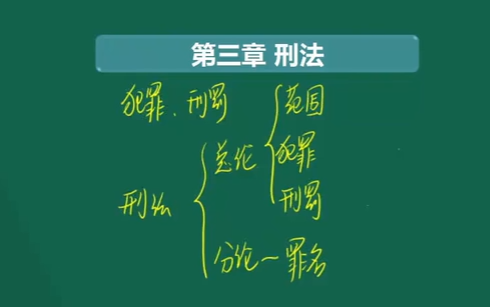
\includegraphics[scale=0.5]{criminal_law_intro}\\ 

%%%%%%%%%%%%%%%%%%%%%%%%%%%%%%%%%%%%%%%%
% support for basic color
%  
% \textcolor{red/blue/green/black/white/cyan/magenta/yellow}{text}
%  
%%%%%%%%%%%%%%%%%%%%%%%%%%%%%%%%%%%%%%%%
\usepackage{color}


%%%%%%%%%%%%%%%%%%%%%%%%%%%%%%%%%%%%%%%%
% support for basic color
%  
% \textcolor{red/blue/green/black/white/cyan/magenta/yellow}{text}
%  
%  \begin{comment}
%  \end{comment}
%%%%%%%%%%%%%%%%%%%%%%%%%%%%%%%%%%%%%%%%
\usepackage{verbatim}

%%%%%%%%%%%%%%%%%%%%%%%%%%%%%%%%%%%%%%%%
 % 常用的符号
%%%%%%%%%%%%%%%%%%%%%%%%%%%%%%%%%%%%%%%%
 %\ approx   约等于

 %   { \scriptsize
 %   
 %   \begin{gather}
 %       \text{销售额} = \frac{\text{总销售额}}{\text{月份数}} \\
 %       = \frac{1}{12} \\
 %       = \frac{12 \times 44 + (123)}{12} \\
 %       \approx 44
 %   \end{gather}
 %                 
 %                 
 %   }
 %


\begin{document}
%
% Basic Information Of This Silde
%

\title{2019 年 6 月广东深圳市属事业单位招聘《行政职业能力测试》真题}
\author{AKA}
\institute{AKA}
\date{\today}

%%%%%%%%%%%%%%%%%%%%%%%%%%%%%%%%%%%%%%%%
% titlepage
%%%%%%%%%%%%%%%%%%%%%%%%%%%%%%%%%%%%%%%%
\begin{frame}
\titlepage
\end{frame}

%%%%%%%%%%%%%%%%%%%%%%%%%%%%%%%%%%%%%%%%%%%%%%%%%%%%%%%%%%%%%%%%%%%%%%%%%%%%%%%%%%%%%%%%%%%%%%%%%%%%%%%%%%%%%%%%%%%%%%%%
  \begin{comment}

%%%%%%%%%%%%%%%%%%%%%%%%%%%%%%%%%%%%%%%%
% A frame
%%%%%%%%%%%%%%%%%%%%%%%%%%%%%%%%%%%%%%%%
\begin{frame}[t]{数量关系}
    \textbf{1、}
    1,1,2,4,7,13,( )\\
    A、15\\
    B、19\\
    C、22\\
    D、24\\
\end{frame}

%%%%%%%%%%%%%%%%%%%%%%%%%%%%%%%%%%%%%%%%
% A frame
%%%%%%%%%%%%%%%%%%%%%%%%%%%%%%%%%%%%%%%%
\begin{frame}[t]{数量关系}
    \textbf{1、}
    1,1,2,4,7,13,( )\\
    A、15\\
    B、19\\
    C、22\\
    D、24\\
    解析:\textcolor{red}{D}\\
    数列无明显特征,多级作差无规律,考虑递推。观察发现:\\
    $1+1+2=4$,\\
    $1+2+4=7$,\\
    $2+4+7=13$,\\
    $4+7+13=24$\\
    即从第四项开始,每一项都等于前三项数字之和\\
\end{frame}


%%%%%%%%%%%%%%%%%%%%%%%%%%%%%%%%%%%%%%%%
% A frame
%%%%%%%%%%%%%%%%%%%%%%%%%%%%%%%%%%%%%%%%
\begin{frame}[t]{数量关系}
    \textbf{2、}-2,-4,0,16,( )
    A、20\\
    B、30\\
    C、40\\
    D、50\\
\end{frame}


%%%%%%%%%%%%%%%%%%%%%%%%%%%%%%%%%%%%%%%%
% A frame
%%%%%%%%%%%%%%%%%%%%%%%%%%%%%%%%%%%%%%%%
\begin{frame}[t]{数量关系}
    \textbf{2、} $-2$,$-4$,0,16,( )\\
    A、20\\
    B、30\\
    C、40\\
    D、50\\
    解析:\textcolor{red}{D}\\
    2、数列无明显特征,多级与递推均无规律,且大部分数为合数,考虑因数分解。原数列可分别分解为:\\
    $-2 \times 1^2$\\
    $-1 \times 2^2$\\
    $0 \times 3^2$\\
    $1 \times 4^2$\\
    $2 \times 5^2$\\
\end{frame}



%%%%%%%%%%%%%%%%%%%%%%%%%%%%%%%%%%%%%%%%
% A frame
%%%%%%%%%%%%%%%%%%%%%%%%%%%%%%%%%%%%%%%%
\begin{frame}[t]{数量关系}
    \textbf{3、}1,1,4,8,9,27,16,( )\\
    A、63\\
    B、64\\
    C、25\\
    D、26\\
\end{frame}


%%%%%%%%%%%%%%%%%%%%%%%%%%%%%%%%%%%%%%%%
% A frame
%%%%%%%%%%%%%%%%%%%%%%%%%%%%%%%%%%%%%%%%
\begin{frame}[t]{数量关系}
    \textbf{3、}1,1,4,8,9,27,16,( )\\
    A、63\\
    B、64\\
    C、25\\
    D、26\\
    解析:\textcolor{red}{B}\\
    数列项数较多,优先考虑多重数列。\\
    奇数项构成平方数列,可以表示为:\\
    $1^2, 2^2, 3^2, 4^2$\\
    偶数项构成立方数列,可以表示为:\\
    $1^3, 2^3, 3^3$\\
    底数是公差为 1 的等差数列, 所求项$=(3+1)^3 = 64$\\
\end{frame}


%%%%%%%%%%%%%%%%%%%%%%%%%%%%%%%%%%%%%%%%
% A frame
%%%%%%%%%%%%%%%%%%%%%%%%%%%%%%%%%%%%%%%%
\begin{frame}[t]{数量关系}
    \textbf{4、}5,11,24,52,( )\\
    A、88 \\
    B、112\\
    C、130\\
    D、156\\
\end{frame}

%%%%%%%%%%%%%%%%%%%%%%%%%%%%%%%%%%%%%%%%
% A frame
%%%%%%%%%%%%%%%%%%%%%%%%%%%%%%%%%%%%%%%%
\begin{frame}[t]{数量关系}
    \textbf{4、}5,11,24,52,( )\\
    A、88 \\
    B、112\\
    C、130\\
    D、156\\
    解析:\textcolor{red}{B}\\
    数列无明显特征,多级无规律,考虑递推。观察发现:\\
    $2 \times 5 = 10, 10+1=11$\\
    $2 \times 11 = 22, 22+2=24$\\
    $2 \times 24 = 48, 48+4=52$\\
    $2 \times 52 = 104, 104+8=112$\\
\end{frame}


%%%%%%%%%%%%%%%%%%%%%%%%%%%%%%%%%%%%%%%%
% A frame
%%%%%%%%%%%%%%%%%%%%%%%%%%%%%%%%%%%%%%%%
\begin{frame}[t]{数量关系}
    \textbf{5、}8,24,16,20,18,( )\\
    A、19\\
    B、20\\
    C、21\\
    D、22\\
\end{frame}

%%%%%%%%%%%%%%%%%%%%%%%%%%%%%%%%%%%%%%%%
% A frame
%%%%%%%%%%%%%%%%%%%%%%%%%%%%%%%%%%%%%%%%
\begin{frame}[t]{数量关系}
    \textbf{5、}8,24,16,20,18,( )\\
    A、19\\
    B、20\\
    C、21\\
    D、22\\
    解析:\textcolor{red}{A}\\
    方法一:数列无明显特征,考虑多级作差。后项减前项,得到新数列:\\
    $16, -8, 4, -2, 1$,构成公比为 $-\frac{1}{2}$的等比数列, 故所求项为$18+1=19$\\
    方 法 二 : 观 察可得: \\
    $(8+24) \div 2 = 16$\\
    $(24+16) \div 2 = 20$\\
    $(20+18) \div 2 = 19$\\
\end{frame}


%%%%%%%%%%%%%%%%%%%%%%%%%%%%%%%%%%%%%%%%
% A frame
%%%%%%%%%%%%%%%%%%%%%%%%%%%%%%%%%%%%%%%%
\begin{frame}[t]{数量关系}
    6、甲,乙两站均为每隔 50 分钟同时对向发一趟客车,客车从甲站到乙站,单程需行驶 4 小时,每辆客车
的行驶速度相同,某旅客乘车从甲站到乙站,他在行程中最多可以遇到从乙站开往甲站的客车( )辆\\
A、10\\
B、9\\
C、8\\
D、5\\
\end{frame}


%%%%%%%%%%%%%%%%%%%%%%%%%%%%%%%%%%%%%%%%
% A frame
%%%%%%%%%%%%%%%%%%%%%%%%%%%%%%%%%%%%%%%%
\begin{frame}[t]{数量关系}
    6、甲,乙两站均为每隔 50 分钟同时对向发一趟客车,客车从甲站到乙站,单程需行驶 4 小时,每辆客车
的行驶速度相同,某旅客乘车从甲站到乙站,他在行程中最多可以遇到从乙站开往甲站的客车( )辆\\
A、10\\
B、9\\
C、8\\
D、5\\
    解析:\textcolor{red}{B},
    单程 4 小时, 即 $4 \times 60 = 240min$ ,
    由于甲乙同时发车, 旅客会遇到在他启程前已经从乙车站出发还没到达的汽车和启程后在乙车站出发的汽车,
    由于每 50 分钟 出发一辆,$240=50+50+50+50+40$ 之前出发未到的车中有一辆还差 40 分钟到达,
    由于速度相同,则乘客出发后 20 分钟可遇到第一辆车,此时还剩下$240-20=220 min$,因为两个车同时走,所以接下的时间每 $(50 \div 2) = 25 min$ 遇到一辆车,
    则$(220 \div 5 ) = 8...20$ 则遇到 8 辆车, 总共遇到 $8+1=9$ 辆车。

\end{frame}



%%%%%%%%%%%%%%%%%%%%%%%%%%%%%%%%%%%%%%%%
% A frame
%%%%%%%%%%%%%%%%%%%%%%%%%%%%%%%%%%%%%%%%
\begin{frame}[t]{数量关系}
    7、某人 2012 的年龄是 3 的倍数,2013 年的年龄是 4 的倍数,2014 年的年龄是 5 的倍数,则此人 2015 年
的年龄是( )岁。\\
A、56\\
B、60\\
C、61\\
D、66\\
    解析:\textcolor{red}{D}\\
    A.2015 年 56 岁,则 2012 年为 $56-3 = 53$,不是 3 的倍数,排除;\\
    B.2015 年 60 岁,则 2012 年为 $60-3 = 57$,是 3 的倍数,2013 年为 $57+1 = 58$,不是 4 的倍数\\
    C.2015 年 61 岁,则 2012 年为 $61-3 = 58$,不是 3 的倍数,排除;\\
    D.2015 年 66 岁,则 2012 年为 $66-3 = 63$,是 3 的倍数,2013 年为 $63+1 = 64$,是 4 的倍数,2014
年为 $63+2 = 65$,是 5 的倍数,正确。\\
\end{frame}



%%%%%%%%%%%%%%%%%%%%%%%%%%%%%%%%%%%%%%%%
% A frame
%%%%%%%%%%%%%%%%%%%%%%%%%%%%%%%%%%%%%%%%
\begin{frame}[t]{数量关系}
8、有十名高级工匠的工号依次为 1——10,若从中调走一名,则其余 9 名的工号的平均值较原来减少了 0.5,
调走的高级工证的工号是( )。\\
A、3\\
B、7\\
C、8\\
D、10\\
\end{frame}



%%%%%%%%%%%%%%%%%%%%%%%%%%%%%%%%%%%%%%%%
% A frame
%%%%%%%%%%%%%%%%%%%%%%%%%%%%%%%%%%%%%%%%
\begin{frame}[t]{数量关系}
8、有十名高级工匠的工号依次为 1——10,若从中调走一名,则其余 9 名的工号的平均值较原来减少了 0.5,
调走的高级工证的工号是( )。\\
A、3\\
B、7\\
C、8\\
D、10\\
    解析:\textcolor{red}{D}\\
    调走前平均值$\frac{(1+2+3+4+5+6+7+8+9+10)}{10} = \frac{55}{10} = 5.5$\\
    调走后平均值$5.5 - 0.5 = 5$, 调走后还剩 9 人,则$(5\times9) = 45$\\
    则调走的人的工号为 $55-45=10$\\
\end{frame}


%%%%%%%%%%%%%%%%%%%%%%%%%%%%%%%%%%%%%%%%
% A frame
%%%%%%%%%%%%%%%%%%%%%%%%%%%%%%%%%%%%%%%%
\begin{frame}[t]{数量关系}
    9、某研究生院今年的研一新生共 1305 人,比去年增加了 4.4\%,其中女生人数减少 4\%,男生人数增加 10\%,
则该院今年的研一新生中有男生( )人。\\
A、790\\
B、805\\
C、825\\
D、865\\
\end{frame}


%%%%%%%%%%%%%%%%%%%%%%%%%%%%%%%%%%%%%%%%
% A frame
%%%%%%%%%%%%%%%%%%%%%%%%%%%%%%%%%%%%%%%%
\begin{frame}[t]{数量关系}
    9、某研究生院今年的研一新生共 1305 人,比去年增加了 4.4\%,其中女生人数减少 4\%,男生人数增加 10\%,
则该院今年的研一新生中有男生( )人。\\
A、790\\
B、805\\
C、825\\
D、865\\
    解析:\textcolor{red}{C}\\
    今年的研一新生共 1305 人,比去年增加了4.4\% ,则去年研一新生总人数$=\frac{1035}{1+4.4\%}= 1250$ \\
    根据线段法,女生与男生人数的增长率的线段距离之比为$\frac{4.4\%-(-4\%)}{10\% - 4.4\%} = \frac{8.4\%}{5.6\%} = \frac{3}{2}$\\
    ,由于增长率线段距离之比与基期量成反比,则有去年女生与男生的人数之比为 2:3,因此去年男生的人数为 $\frac{1250}{2+3} \times 3 = 750$,
    则今年的研一新生中男生人数为 $750 \times (1+10\%) = 825$ \\
\end{frame}

%%%%%%%%%%%%%%%%%%%%%%%%%%%%%%%%%%%%%%%%
% A frame
%%%%%%%%%%%%%%%%%%%%%%%%%%%%%%%%%%%%%%%%
\begin{frame}[t]{数量关系}
    9、某研究生院今年的研一新生共 1305 人,比去年增加了 4.4\%,其中女生人数减少 4\%,男生人数增加 10\%,
则该院今年的研一新生中有男生( )人。\\
A、790\\
B、805\\
C、825\\
D、865\\
    解析:\textcolor{red}{C}\\
    方法二: 今年的研一新生男生数 = 去年男生数 $\times (1+10\%)  = 1.1 \times $ 去年男生数,即 
    今年男生人数/去年男生人数 $= \frac{11}{10}$ \\
人数必须为整数,所以今年男生人数必须为 11 的倍数,仅 C 项符合。\\
\end{frame}




%%%%%%%%%%%%%%%%%%%%%%%%%%%%%%%%%%%%%%%%
% A frame
%%%%%%%%%%%%%%%%%%%%%%%%%%%%%%%%%%%%%%%%
\begin{frame}[t]{数量关系}
    10、某项目由甲乙二人竞标,以所报单价高者胜,甲从 10 元,11 元,12 元,13 元,16 元,17 元六个单
价中随机选择一个作为合作价,乙从 13 元,14 元,15 元中随机选取一个作为报价,则乙中标的概率为( )。\\
    A、$\frac{7}{18}$  \\
    B、$\frac{11}{18}$ \\
    C、$\frac{2}{3} $  \\
    D、$\frac{5}{6} $  \\
\end{frame}


%%%%%%%%%%%%%%%%%%%%%%%%%%%%%%%%%%%%%%%%
% A frame
%%%%%%%%%%%%%%%%%%%%%%%%%%%%%%%%%%%%%%%%
\begin{frame}[t]{数量关系}
    10、某项目由甲乙二人竞标,以所报单价高者胜,甲从 10 元,11 元,12 元,13 元,16 元,17 元六个单
价中随机选择一个作为合作价,乙从 13 元,14 元,15 元中随机选取一个作为报价,则乙中标的概率为( )。\\
    A、$\frac{7}{18}$  \\
    B、$\frac{11}{18}$ \\
    C、$\frac{2}{3} $  \\
    D、$\frac{5}{6} $  \\
    解析:\textcolor{red}{C}\\
    根据概率公式 $p=$ 满足总情况数/总数, 甲有 6 种报价方式,乙有 3 种报价方式,则总数为 种,满足
条件的情况数有以下几种\\
乙报价为 13 元,甲报价为 10 元,11 元,12 元时,乙可以中标,共 3 种情况;\\
乙报价为 14 元,甲报价为 10 元,11 元,12 元,13 元时,乙可以中标,共 4 种情况;\\
乙报价为 15 元,甲报价为 10 元,11 元,12 元,13 元时,乙可以中标,共 4 种情况\\
    因此乙能中标的情况为 $3+4+4 = 11$ 种, 则 概率 $p=\frac{11}[18]$\\

\end{frame}



%%%%%%%%%%%%%%%%%%%%%%%%%%%%%%%%%%%%%%%%
% A frame
%%%%%%%%%%%%%%%%%%%%%%%%%%%%%%%%%%%%%%%%
\begin{frame}[t]{言语理解}
    11、仅仅把环境保护理解为人“聪明的自利”,尊重和维护自然的全部目的也仅仅是为了人的利
    益,这样的思想也()有些狭隘了\\
A、不免\\
B、未免\\
C、难免\\
D、以免\\
\end{frame}

%%%%%%%%%%%%%%%%%%%%%%%%%%%%%%%%%%%%%%%%
% A frame
%%%%%%%%%%%%%%%%%%%%%%%%%%%%%%%%%%%%%%%%
\begin{frame}[t]{言语理解}
    11、仅仅把环境保护理解为人“聪明的自利”,尊重和维护自然的全部目的也仅仅是为了人的利
    益,这样的思想也()有些狭隘了\\
A、不免 \qquad B、未免\\
C、难免 \qquad  D、以免\\
    解析:\textcolor{red}{B}\\
“这样的思想”指代的是前文“仅仅把环境保护……,尊重和维护自然的全部目的也仅仅是……”,
由“仅仅”可知,这样的思想确实片面、狭隘,故横线处应对前文观点予以否定,B 项,“未免”意为实在是,
不能不说是,多指人对过分的事情不以为然,或委婉给予否定的评价,符合文意,当选。
A 项,“不免”意为避免不了或难以避免,并非对前文观点语义否定,排除。
C 项,“难免”强调的是某种结果不容易避免,多用于规律性情况或有一种解释或宽慰的语气,暗含没什
么,事情不严重之意,文中并未有思想狭隘不严重之意,排除。
D 项,“以免”多用于提起下半句话,表明前半句话是为了使下半句话所说的情形不至于发生,填入后与
文意相悖,排除。
\end{frame}


%%%%%%%%%%%%%%%%%%%%%%%%%%%%%%%%%%%%%%%%
% A frame
%%%%%%%%%%%%%%%%%%%%%%%%%%%%%%%%%%%%%%%%
\begin{frame}[t]{言语理解}
    12、将下列选项中的词语依次填入各句横线处,最恰当的一组是:\\
    (1)生活中的长久沉积,犹如陈年佳酿,其味越来越()、绵长。\\
   (2)只见他神情自若地从口袋里掏出窃来的讲稿,对着在座的教授们口若悬河、()地讲开了。\\
\textbf{A}醇正,振振有词
\textbf{B}醇正,念念有词
\textbf{C}纯正,振振有词
\textbf{D}纯正,念念有词\\
 解析:\textcolor{red}{A}
    第(1)句,横线处用  来形容陈年佳酿的味道,A、B 项的“醇正”指酒的品质厚重柔和,不仅正宗绵
甜,而且回味悠长,可与“陈年佳酿”搭配,保留。C、D 项的“纯正”指纯粹;不搀杂其他成分,多与“性情、
品格”等搭配,用于此处不当,排除;
第(2)句,横线处需与“口若悬河”构成并列,且对应前文的“窃来的讲稿”,故横线处应填入表示不停
说话或说很多的贬义词,A 项“振振有词”意为理直气壮的样子。借以形容自以为理由充分,说个没完。多用
作贬义。符合文意,当选。B 项“念念有词”旧指迷信的人祈祷时不停地念着口语,以通神灵,现多用来形容
人嘟嘟囔囔说个不停。填入横线处感情色彩不如 A 项恰当,对比择优,排除
\end{frame}



%%%%%%%%%%%%%%%%%%%%%%%%%%%%%%%%%%%%%%%%
% A frame
%%%%%%%%%%%%%%%%%%%%%%%%%%%%%%%%%%%%%%%%
\begin{frame}[t]{言语理解}
    13、将下列选项中的词语依次填入各句横线处,最恰当的一组是:\\
    (1)精灵鬼怪,花草树木,宫殿楼阁都在这个()的世界里被安徒生的妙笔赋予了生命。\\
    (2)从前研究中国文化的人,往往只看高层次的思想,意识形态,而忽视了现实生活中很多和观念文化理
    想冲突的方面,这样的文化研究者,就是犯了()的错误。\\
    A、光怪陆离,目无全牛\\
    B、光怪陆离,以偏概全\\
    C、斑驳陆离,目无全牛\\
    D、斑驳陆离,以偏概全\\
\end{frame}



%%%%%%%%%%%%%%%%%%%%%%%%%%%%%%%%%%%%%%%%
% A frame
%%%%%%%%%%%%%%%%%%%%%%%%%%%%%%%%%%%%%%%%
\begin{frame}[t]{言语理解}
 解析:\textcolor{red}{B}\\
    第一空,修饰“安徒生的童话世界”,“光怪陆离”形容事物离奇多变,奇形怪状、五颜六色,对应
前文“精灵鬼怪,花草树木,宫殿楼阁”,体现出安徒生的童话世界多样精彩,A、B 两项保留;\\
    “斑驳陆离”
形容颜色繁杂、斑驳绚丽,不能与童话世界搭配,排除 C、D 两项。\\

第二空,搭配“错误”,感情色彩消极,B 项“以偏概全”指用片面的观点看待整体问题,感情色彩消极,
符合文意,当选;\\
    A 项“目无全牛”比喻技术熟练到了得心应手的境地,感情色彩积极褒义,排除。
故正确答案为 B
\end{frame}



%%%%%%%%%%%%%%%%%%%%%%%%%%%%%%%%%%%%%%%%
% A frame
%%%%%%%%%%%%%%%%%%%%%%%%%%%%%%%%%%%%%%%%
\begin{frame}[t]{言语理解}
14、将下列选项中的词语依次填入句子横线处,最恰当的一组是:\\
    在小数据时代,人们可以通过数据和分析来验证猜想,以上世纪 80 年代文学为例,文学()能成为
    社会热点。与文学生产相对有限且思想表现集中在思想启蒙上有直接关系,()与出版流通相对缓慢有关。\\
    如研究改革文学,彼时的文学批评者完全可以穷尽有限的文本。()遗漏一些文本,批评家()可
以言之凿凿,所作的推论基本有效。\\
A、一方面,另一方面,尽管,还是\\
B、一方面,另一方面,如果,就\\
C、之所以,还,即便,仍然\\
D、之所以,还,只要,就\\
\end{frame}


%%%%%%%%%%%%%%%%%%%%%%%%%%%%%%%%%%%%%%%%
% A frame
%%%%%%%%%%%%%%%%%%%%%%%%%%%%%%%%%%%%%%%%
\begin{frame}[t]{言语理解}
    解析:\textcolor{red}{C}\\
    14、根据“在思想启蒙上有直接关系”可知,“出版流通相对缓慢有关”是文学能成为社会热点的第二个
原因,故前两空之间应该填入因果关系的关联词,对应 C、D 项保留;\\
    “一方面……另一方面”为并列关系,排除 A、B 两项。\\
    第二空,前文“遗漏文本”,后文批评家的推论还是能够有效,说明两句话之间存在假设关系,
即便遗漏一些文本,仍然可以言之凿凿,推论基本有效,对应 C 项,当选;D 项“只要……就”为条件关系,
不符合文段逻辑,排除。
故正确答案为 C
\end{frame}



%%%%%%%%%%%%%%%%%%%%%%%%%%%%%%%%%%%%%%%%
% A frame
%%%%%%%%%%%%%%%%%%%%%%%%%%%%%%%%%%%%%%%%
\begin{frame}[t]{言语理解}
15、将下列选项中的词语依次填入各句横线处,最恰当的一组是:\\
    (1)如今,企业经营者们都多了一些理性的思考和判断,盲目炒卖房地产的现象有所缓解。而() 的房地产公司已自消自灭,一些无经营实力,想玩“空手道”的公司也难以得手。\\
(2)他用行动证明了只要肯付诸行动,不怕90,而且有毅力坚持下去,天底下就没有战不胜的困
难。\\
A、出风头,碰钉子\\
B、出风头,敲竹杠\\
C、赶浪头,敲竹杠\\
D、赶浪头,碰钉子\\
\end{frame}

%%%%%%%%%%%%%%%%%%%%%%%%%%%%%%%%%%%%%%%%
% A frame
%%%%%%%%%%%%%%%%%%%%%%%%%%%%%%%%%%%%%%%%
\begin{frame}[t]{言语理解}
    解析:\textcolor{red}{D}\\
    15、第一空,根据“盲目炒卖房地产的现象有所缓解”可知,横线处填入词语应体现出房地产公司借机敛
财之意,“赶浪头”指比喻紧紧追随时尚,做适应当前形势的事,符合文意。“出风头”指出头露面显示自己,
与文意无关,故排除 A、B 两项。\\
第二空,根据“天底下就没有战不胜的困难”可知,横线处词语应体现出困难之意,D 项“碰钉子”比喻
遭到拒绝或受到斥责,有遇到困难的意思。C 项“敲竹杠”指利用别人的弱点或借某种口实抬高价格或索取财
物,与文意无关,排除。\\
故正确答案为 D\\
\end{frame}



%%%%%%%%%%%%%%%%%%%%%%%%%%%%%%%%%%%%%%%%
% A frame
%%%%%%%%%%%%%%%%%%%%%%%%%%%%%%%%%%%%%%%%
\begin{frame}[t]{言语理解}
16、下列各句中,没有语病的是( )。\\
A、历代古今中外的经验证明,教育孩子要重视榜样的作用,特别是家长的榜样作用。\\
B、经过市立学院几位专家的指导,让该市葡萄的产量和质量都得到了很大的改善。\\
C、有少数观众素质不高,当参赛选手出现因过度紧张而未正常发挥技术或有所失误时,便嘘声四起。\\
D、据统计,“好读书”基金在过去的十余年里,一共积累了逾千万元的助学奖金。\\
\end{frame}

%%%%%%%%%%%%%%%%%%%%%%%%%%%%%%%%%%%%%%%%
% A frame
%%%%%%%%%%%%%%%%%%%%%%%%%%%%%%%%%%%%%%%%
\begin{frame}[t]{言语理解}
    解析:\textcolor{red}{D}\\
    16、A 项,“历代”赘余,因“古今中外”即含有“历代”的意思,排除;\\
    B 项,“经过……让”缺少主语,成分残缺,排除;\\
    C 项,语序不当,“因过度紧张而”作为状语,应在“出现”之前,且“出现”与“未正常发挥技术”不
    能搭配使用,应为“出现未正常发挥技术的情况”,排除;\\
    D 项,表述正确,当选。\\
    故正确答案为 D\\
\end{frame}




%%%%%%%%%%%%%%%%%%%%%%%%%%%%%%%%%%%%%%%%
% A frame
%%%%%%%%%%%%%%%%%%%%%%%%%%%%%%%%%%%%%%%%
\begin{frame}[t]{言语理解}
17、下列各句中,有语病的是( )。\\
A、我国的经济发展仍处于可以大有作为的重要战略机遇期,蕴藏着巨大的潜力。\\
B、过去七年中,无良的汽车厂家在大约 1100 万辆柴油汽车上安装作弊软件以通过尾气排放检测。\\
C、虽然十分疲惫,但一想起几个月来一连串发生的怪事,那个老农民怎么也睡不着了。\\
D、“十三五”期间,生育政策作为备受关注的一项公共政策,其可能发生的变化值得各方期待。\\
\end{frame}



%%%%%%%%%%%%%%%%%%%%%%%%%%%%%%%%%%%%%%%%
% A frame
%%%%%%%%%%%%%%%%%%%%%%%%%%%%%%%%%%%%%%%%
\begin{frame}[t]{言语理解}
    17、下列各句中,有语病的是( )。\\
    A、我国的经济发展仍处于可以大有作为的重要战略机遇期,蕴藏着巨大的潜力。\\
    B、过去七年中,无良的汽车厂家在大约 1100 万辆柴油汽车上安装作弊软件以通过尾气排放检测。\\
    C、虽然十分疲惫,但一想起几个月来一连串发生的怪事,那个老农民怎么也睡不着了。\\
    D、“十三五”期间,生育政策作为备受关注的一项公共政策,其可能发生的变化值得各方期待。\\

    解析:\textcolor{red}{C}\\
    C 项,定语误放在状语位置,应改为“发生的一连串怪事”,故语序不当,当选;\\
    A 项、B 项、D 项,均表述正确,排除。\\
    本题为选非题,故正确答案为 C\\
\end{frame}



%%%%%%%%%%%%%%%%%%%%%%%%%%%%%%%%%%%%%%%%
% A frame
%%%%%%%%%%%%%%%%%%%%%%%%%%%%%%%%%%%%%%%%
\begin{frame}[t]{言语理解}
18、说到这个问题,他从资料箱里拿出十几封信,其中一封来自 S 区保安大队全体保安写的。以上句子所
属的语病类型是( )。\\
A、成分残缺\\
B、句式杂糅\\
C、语序不当\\
D、搭配不当 \\
\end{frame}


%%%%%%%%%%%%%%%%%%%%%%%%%%%%%%%%%%%%%%%%
% A frame
%%%%%%%%%%%%%%%%%%%%%%%%%%%%%%%%%%%%%%%%
\begin{frame}[t]{言语理解}
18、说到这个问题,他从资料箱里拿出十几封信,其中一封来自 S 区保安大队全体保安写的。以上句子所
属的语病类型是( )。\\
A、成分残缺\\
B、句式杂糅\\
C、语序不当\\
D、搭配不当 \\
    解析:\textcolor{red}{B}\\
    文中语句可以说“说到这个问题,他从资料箱里拿出十几封信,其中一封来自 S 区保安大队全体保安”,
也可以说“说到这个问题,他从资料箱里拿出十几封信,其中一封是 S 区保安大队全体保安写的”,故本句属
于句式杂糅的错误。\\
故正确答案为 B\\
\end{frame}




%%%%%%%%%%%%%%%%%%%%%%%%%%%%%%%%%%%%%%%%
% A frame
%%%%%%%%%%%%%%%%%%%%%%%%%%%%%%%%%%%%%%%%
\begin{frame}[t]{言语理解}
19、下列各句中,有语病的是( )。\\
A、这是一座跨越了一千五百年的老建筑,在这里,哥特式风格与伊斯兰风格完美融合,营造出西班牙所特
有的人文环境。\\
B、未成年人保护观念的进步使得赖宁精神逐渐被淡化,但谁又能否认现在依然需要学习赖宁呢?\\
C、国际移民组织已启动一项旨在从几个方面帮助战后伊拉克重建的人道主义援助计划。\\
D、蛞蝓是一种高蛋白、低脂肪、营养丰富的软体动物,肉味光滑、白润,含有多种氨基酸、酶类和维生素,\\
还具有一定的药用功效。\\
\end{frame}


%%%%%%%%%%%%%%%%%%%%%%%%%%%%%%%%%%%%%%%%
% A frame
%%%%%%%%%%%%%%%%%%%%%%%%%%%%%%%%%%%%%%%%
\begin{frame}[t]{言语理解}
19、下列各句中,有语病的是( )。\\
A、这是一座跨越了一千五百年的老建筑,在这里,哥特式风格与伊斯兰风格完美融合,营造出西班牙所特
有的人文环境。\\
B、未成年人保护观念的进步使得赖宁精神逐渐被淡化,但谁又能否认现在依然需要学习赖宁呢?\\
C、国际移民组织已启动一项旨在从几个方面帮助战后伊拉克重建的人道主义援助计划。\\
D、蛞蝓是一种高蛋白、低脂肪、营养丰富的软体动物,肉味光滑、白润,含有多种氨基酸、酶类和维生素,\\
还具有一定的药用功效。\\
    解析:\textcolor{red}{B}\\
    D 项“肉味”与“光滑、白润”搭配不当,可改为“肉味鲜美”。\\
故正确答案为 D。\\
\end{frame}




%%%%%%%%%%%%%%%%%%%%%%%%%%%%%%%%%%%%%%%%
% A frame
%%%%%%%%%%%%%%%%%%%%%%%%%%%%%%%%%%%%%%%%
\begin{frame}[t]{言语理解}
20、把下面几个句子组成语意连贯的一段文字,排序正确的一项是( )。\\
(1)由于画院画家的风格过于近似。\\
(2)甚至假定越精彩、越优秀的画作越有可能出自徽宗皇帝之手也未必准确\\
(3)徽宗每创作一副精品,画院画家们便争相模仿\\
(4)尽管有过不少尝试,但事实上很难将他们的作品区分开来\\
(5)如果他们足够幸运,皇帝就会在他们画作上题签以示确认\\
A、3-5-1-4-2\\
B、3-5-4-2-1\\
C、1-4-2-3-5\\
D、1-3-5-4-2\\
\end{frame}



%%%%%%%%%%%%%%%%%%%%%%%%%%%%%%%%%%%%%%%%
% A frame
%%%%%%%%%%%%%%%%%%%%%%%%%%%%%%%%%%%%%%%%
\begin{frame}[t]{言语理解}
    解析:\textcolor{red}{A}\\
对比首句,1 句指出画院画家风格相似,3 句指出画院画家们便争相模仿徽宗的画作精品。对比两句发
现,应是画家们争相模仿一样的画作才导致他们风格相似,故 3 句应在 1 句之前,排除 C、D 项。\\
对比 A、B 项,判别 1 句与 4 句顺序,应是由于画家风格相似才产生画家的作品难以区别的结果,故 1 句应
在 4 句之前,排除 B 项,锁定 A 项。\\
故正确答案为 A
\end{frame}





%%%%%%%%%%%%%%%%%%%%%%%%%%%%%%%%%%%%%%%%
% A frame
%%%%%%%%%%%%%%%%%%%%%%%%%%%%%%%%%%%%%%%%
\begin{frame}[t]{言语理解}
21、溃疡病是一种常见的多因性疾病。在人体中一切器官都受到大脑管理,胃也包括其中。如果大脑皮层
受到某种有害刺激,其机能就会降低,比较低级的神经中枢的机能反而亢进,导致胃酸分泌增多,胃部肌肉紧
张性加强,供应胃血液的血管痉挛。由于一方面胃酸增加,一方面胃粘膜细胞血液供应不良,导致部分胃被消
化形成溃疡。长期溃疡病的疼痛刺激会影响并加重大脑皮层功能紊乱,进一步加重溃疡病,从而形成恶性循环。
临床实践中,因精神紧张、过度疲劳、恐惧忧伤等精神异常引起溃疡病发生且加重者屡见不鲜。如二战期间,
一些城市和军队溃疡病发生率明显升高,二战结束后,溃疡也迅速愈合了。\\
这段文字主要说明的是( )。\\
A、精神因素导致溃疡病产生的机制\\
B、二战期间溃疡病发生率升高的原因\\
C、胃溃疡产生的生理基础\\
D、精神健康是促使溃疡病痊愈的关键\\
\end{frame}


%%%%%%%%%%%%%%%%%%%%%%%%%%%%%%%%%%%%%%%%
% A frame
%%%%%%%%%%%%%%%%%%%%%%%%%%%%%%%%%%%%%%%%
\begin{frame}[t]{言语理解}
    解析:\textcolor{red}{A}\\
    文段开篇引出“溃疡病”这一话题,紧接着指出胃受到大脑管理,大脑皮层受刺激后,会导致溃疡病
产生甚至加重。并通过临床实践及二战期间的相关事例进行论证。故整个文段均在说明精神因素会导致溃疡病
的产生展开,对应 A 项。\\
B 项,“二战期间溃疡病发生率升高”对应后文举例说明的内容,非重点,排除;\\
C 项,“胃溃疡产生的生理基础”表述不明确,文段明确指出是精神因素导致溃疡病的产生,排除;\\
D 项,文段重点强调大脑皮层受到某种有害刺激,即精神紧张、大脑疲惫、恐惧忧伤等时会导致溃疡病产
生,并未明确指出溃疡病痊愈的关键,且“精神健康”仅对应“精神紧张”这一种刺激,表述片面,排除。\\
故正确答案为 A。\\
\end{frame}




%%%%%%%%%%%%%%%%%%%%%%%%%%%%%%%%%%%%%%%%
% A frame
%%%%%%%%%%%%%%%%%%%%%%%%%%%%%%%%%%%%%%%%
\begin{frame}[t]{言语理解}
22、行书的产生也是很早的,某种程度上可以说是与楷书、草书同时产生,因为所谓“行楷”“行草”,
只是很模糊的概念,没有绝对的界限。但是到了这三大书体各自成熟之后,彼此的风格与特点还是判然可分的。
无论如何,大概在魏晋时代,行书就开始在民间流行了。20 世纪初,我国新疆地区古楼兰国遗址出土了大量的
魏晋文书残纸,里头有不少已经是相当成熟的行书了。被称为“书圣”的东晋大书法家王羲之创作了大量的行
书作品,长期以来备受后人的珍爱。\\
下列说法与原文意思相符的是( )。\\
A、“行楷”“行草”没有绝对的界限,所以两者是同时产生的\\
B、成熟的行书、楷书和草书都是具有独特的风格与鲜明的特点\\
C、古楼兰国遗址出土的文书残纸说明在魏晋时行书已经普及\\
D、王羲之创作的行书属于相当成熟的行书作品,因此备受后人喜爱\\
\end{frame}



%%%%%%%%%%%%%%%%%%%%%%%%%%%%%%%%%%%%%%%%
% A frame
%%%%%%%%%%%%%%%%%%%%%%%%%%%%%%%%%%%%%%%%
\begin{frame}[t]{言语理解}
    解析:\textcolor{red}{B}\\
    、A 项,与文中“行书的产生也是很早的,某种程度上可以说是与楷书、草书同时产生,因为所谓“行
楷”“行草”,只是很模糊的概念,没有绝对的界限”对应,文段指出的是在某种程度上,行书与楷书、草书
同时产生,而并未提及“行楷”、“行草”产生的时间,与文意不符,排除;\\
B 项,对应文中“到了这三大书体各自成熟之后,彼此的风格与特点还是判然可分的”,表述正确,当选;\\
C 项,根据文中“我国新疆地区古楼兰国遗址出土了大量的魏晋文书残纸,里头有不少已经是相当成熟的
行书了”可知,出土的魏晋文书残纸仅能证明在魏晋时期行书比较成熟,而普及与否文段未提及,与文意不符,
排除;\\
D 项,与文中“被称为‘书圣’的东晋大书法家王羲之创作了大量的行书作品,长期以来备受后人的珍爱”
对应,文段未提及王羲之的行书备受后人喜爱的原因,与文意不符,排除。\\
故正确答案为 B。\\
\end{frame}





%%%%%%%%%%%%%%%%%%%%%%%%%%%%%%%%%%%%%%%%
% A frame
%%%%%%%%%%%%%%%%%%%%%%%%%%%%%%%%%%%%%%%%
\begin{frame}[t]{言语理解}
23、博物学家的幸福在某种程度上也依靠他的无知,无知给他留下这类新天地让他去征服。他可能在书本
上已经达到了知识的顶峰,但,在他用自己的眼睛证实每一个光辉的细节之前,他仍然感到是半无知的。
根据上文,下列对博物学家的分析正确的是( )。\\
A、博物学家因无知而能达到知识的顶峰\\
B、博物学家在一般人眼中其实也很无知\\
C、博物学家感到无知是因为所掌握的知识不切实际\\
D、博物学家因拥有新天地去征服而感到幸福\\
\end{frame}




%%%%%%%%%%%%%%%%%%%%%%%%%%%%%%%%%%%%%%%%
% A frame
%%%%%%%%%%%%%%%%%%%%%%%%%%%%%%%%%%%%%%%%
\begin{frame}[t]{言语理解}
    解析:\textcolor{red}{D}\\
    A 项,与文中“他可能在书本上已经达到了知识的顶峰”对应,文段并未说明无知与达到知识顶峰之
间存在因果关系,与文意不符,排除;\\
B 项,“博物学家在一般人眼中其实也很无知”,文段未提及,无中生有,排除;\\
C 项,与文中“在他用自己的眼睛证实每一个光辉的细节之前,他仍然感到是半无知的”对应,文段明确
指出,博物学家感到无知的原因是没有亲眼证实这些知识,并非掌握的知识不切实际,与文意不符,排除;\\
D 项,对应文中“博物学家的幸福在某种程度上也依靠他的无知,无知给他留下这类新天地让他去征服”,
表述正确,当选。\\
故正确答案为 D\\
\end{frame}




%%%%%%%%%%%%%%%%%%%%%%%%%%%%%%%%%%%%%%%%
% A frame
%%%%%%%%%%%%%%%%%%%%%%%%%%%%%%%%%%%%%%%%
\begin{frame}[t]{言语理解}
24、中国手工艺复兴是建立在传统文化复兴基础上的:喝茶、焚香、赏花、弹琴、作诗、论字画、把玩瓷
器、收藏古玩、穿中式衣服、摆中式家具,等等。这种生活方式已经在中国的白领阶层中形成新的时尚,也成
为了陶冶性情的一种方式。所谓,“器以载道”,正是这种新的时尚和新的陶冶性情的方式,为手工艺的复兴
打开了出路。而这些具有传统意味又有当代文人风尚的手工艺品的制作者,并非都是传统的手工艺人。其中包
括了那些从美院毕业的富有创造力的年轻艺术家们及设计师们,他们正在利用传统的手工技艺和传统的文化资
源创造新的中国时尚文化,这和民国时期梁漱溟“旧文化转变出一个新文化来”的理想何其相似。许多的传统
手工艺里还蕴含着“中国文化有形的根”而在这样的根底基础上创造出的器物文化与传统中国人“过日子的方
法”具有许多相通之处。\\
\end{frame}


%%%%%%%%%%%%%%%%%%%%%%%%%%%%%%%%%%%%%%%%
% A frame
%%%%%%%%%%%%%%%%%%%%%%%%%%%%%%%%%%%%%%%%
\begin{frame}[t]{言语理解}
下列说法与原文意思不符的是( )。\\
A、喝茶、焚香、赏花、弹琴、作诗、论字画等传统文化的复兴,为手工艺的复兴打开了出路\\
B、传统手艺人与美院毕业的艺术家,设计师都制作出了既有传统意味又有当代文人风尚的手工艺品\\
C、当代人通过利用传统的手工技艺和文化资源创造新的中国时尚文化,实现了梁漱溟“旧文化转变出个新
文化来”的理想\\
D、根植于中国文化的传统手工艺所创造出的器物文化,与传统中国人“过日子的方法”具有许多相通之处\\

\end{frame}



%%%%%%%%%%%%%%%%%%%%%%%%%%%%%%%%%%%%%%%%
% A frame
%%%%%%%%%%%%%%%%%%%%%%%%%%%%%%%%%%%%%%%%
\begin{frame}[t]{言语理解}
    解析:\textcolor{red}{C}\\
    A 项,对应文中“中国手工艺复兴是建立在传统文化复兴基础上的:喝茶、焚香、赏花、弹琴、作诗、
论字画、把玩瓷器、收藏古玩、穿中式衣服、摆中式家具,等等”,表述正确,排除;\\
B 项,根据文中“这些具有传统意味又有当代文人风尚的手工艺品的制作者,并非都是传统的手工艺人。
其中包括了那些从美院毕业的富有创造力的年轻艺术家们及设计师们”可知,选项表述正确,排除;\\
C 项,与文中“这和民国时期梁漱溟‘旧文化转变出一个新文化来’的理想何其相似”对应,文中说明当
代人创造新的中国时尚文化和梁漱溟的理想相似,而并非实现梁漱溟的理想,与文意不符,当选。\\
D 项,对应文中“许多的传统手工艺里还蕴含着‘中国文化有形的根’而在这样的根底基础上创造出的器
物文化与传统中国人“过日子的方法”具有许多相通之处”,表述正确,排除。\\
本题为选非题,故正确答案为 C\\
\end{frame}






%%%%%%%%%%%%%%%%%%%%%%%%%%%%%%%%%%%%%%%%
% A frame
%%%%%%%%%%%%%%%%%%%%%%%%%%%%%%%%%%%%%%%%
\begin{frame}[t]{言语理解}

25、果脯之所以会出现,是因为水果本身有季节性的特点,不耐保鲜,而果脯则一年四季都可以享用。在
不少人的心里,以为一般的果脯就是把鲜果晾晒制成的。其实果脯的制作是一个较为复杂的过程,需要经过脱
水等多项工艺的处理。虽然很多水果本身很甜,但是在加工过程中,为了保证口感,还会再加入大量的糖。如
此处理,水果中原本含有的水溶性维生素 C 大量流失,而热量超高的糖分却大大增加了。因此,果脯不能长期
过量食用,因为摄入过多的糖分,会导致人体中 B 族维生素和某些微量元素的缺乏。尤其是儿童,在饭前更不
宜食用果脯,否则还会影响食欲。另外,有些果脯中可能还含有防腐剂、色素,经常食用会造成这些物质在机
体内的积累,也会影响健康。\\
\end{frame}



%%%%%%%%%%%%%%%%%%%%%%%%%%%%%%%%%%%%%%%%
% A frame
%%%%%%%%%%%%%%%%%%%%%%%%%%%%%%%%%%%%%%%%
\begin{frame}[t]{言语理解}
从这段文字可以推出( )。\\
A、果脯是把鲜果晾晒制成的食品,因耐保鲜而一年四季都可食用\\
B、加工过程中大量添加的糖使得加工后的果脯热量比加工前的水果热量高\\
C、儿童食用果脯会因 B 族维生素和某些微量元素的缺乏而食欲不振\\
D、如果果脯中不添加防腐剂和色素,它将是水果的完美替代品\\

\end{frame}



%%%%%%%%%%%%%%%%%%%%%%%%%%%%%%%%%%%%%%%%
% A frame
%%%%%%%%%%%%%%%%%%%%%%%%%%%%%%%%%%%%%%%%
\begin{frame}[t]{言语理解}
    解析:\textcolor{red}{B}\\
    依据文段“如此处理……热量超高的糖分却大大增加了”可知 B 项表述正确,当选。\\
A 项依据文段“其实果脯的制作是一个较为复杂的过程,需要经过脱水等多项工艺的处理”可知,“果脯
是把鲜果晾晒制成的食品”表述与文意不符,排除;\\
C 项“因 B 族维生素和某些微量元素的缺乏而食欲不振”该因果关系文段未提及,强加因果,排除;\\
D 项“它将是水果的完美替代品”无中生有,排除。\\
故正确答案为 B
\end{frame}



%%%%%%%%%%%%%%%%%%%%%%%%%%%%%%%%%%%%%%%%
% A frame
%%%%%%%%%%%%%%%%%%%%%%%%%%%%%%%%%%%%%%%%
\begin{frame}[t]{言语理解}
26、真言就是说出诗人内心的真话,也许这是一句从来没有人说过的话,也许这句话有悖常理,但是诗人
说出来了:黑夜给了我一双黑色的眼睛,我用它去寻找光明。说出了字面后面更深刻的真实!有人说诗歌就是“废
话”,意思是说诗的语言在现实生活中没有实用性,是无用之言说。这种无用是对“柴米油盐”的无用,却是
精神的佳肴。一首好诗,往往是许多行“废话”蕴藏的一句真话。全部都是真话的不是好诗,而在人们通常视
为废话的诗句里面,包含了诗歌的全部艺术精华。诗歌是废话的艺术,废话不是假话,废话里躲藏真话,像砂
子里的金子,更像树林里的精灵。正因为如此诗人才是语言的炼金师,诗人不断地创造出新的言语。
以下对“全部都是真话的不是好诗”的理解,正确的是( )。\\
A、有一些假话的诗才是好诗\\
B、真话中藏着一些废话才是好诗\\
C、讲究语言锤炼的诗人才是好诗人\\
D、不会创造新语言的诗人不是好诗人\\
\end{frame}


%%%%%%%%%%%%%%%%%%%%%%%%%%%%%%%%%%%%%%%%
% A frame
%%%%%%%%%%%%%%%%%%%%%%%%%%%%%%%%%%%%%%%%
\begin{frame}[t]{言语理解}
以下对“全部都是真话的不是好诗”的理解,正确的是( )。\\
A、有一些假话的诗才是好诗\\
B、真话中藏着一些废话才是好诗\\
C、讲究语言锤炼的诗人才是好诗人\\
D、不会创造新语言的诗人不是好诗人\\
\end{frame}





%%%%%%%%%%%%%%%%%%%%%%%%%%%%%%%%%%%%%%%%
% A frame
%%%%%%%%%%%%%%%%%%%%%%%%%%%%%%%%%%%%%%%%
\begin{frame}[t]{言语理解}
    解析:\textcolor{red}{B}\\
    先定位文段,“全部都是真话的不是好诗”该句出现在文段中间,需要结合前后文内容理解。文段开
头引出话题“真言就是诗人内心真话”并指出其有悖常理,接着转折词“但”强调“诗人的话有深刻的真实”,
接着指出有些人的观点“诗歌就是‘废话’”,接着这通过转折词“却”强调“诗歌里的无用之言是精神佳肴”,
并指出一首好诗即“废话中蕴含真话”。再结合后文“人们视为废话的诗句里,包含了诗歌全部的艺术精华”
以及“废话里藏着真话”,故可知“好诗需要既有真话也有废话”,对应 B 项。\\
A 项“有一些假话的诗才是好诗”与文中“废话不是假话”文意相悖,排除;\\
C、D 两项核心话题为“诗人”与提问“诗”不一致,且该两项均在说明好诗带来的结果,并非对好诗本身
的理解,排除。\\
故本题正确答案为 B\\
\end{frame}



%%%%%%%%%%%%%%%%%%%%%%%%%%%%%%%%%%%%%%%%
% A frame
%%%%%%%%%%%%%%%%%%%%%%%%%%%%%%%%%%%%%%%%
\begin{frame}[t]{言语理解}
27、自互联网技术应用于传媒领域以来,阅读的碎片化以及浅表性问题就不断地招致各种批评,许多有识
之士表达了深切的忧虑。本人也曾在一些撰文中,为碎片化阅读的泛滥痛心疾首、大声疾呼。不过,平心静气
去想,人类社会的阅读历史其实正是由碎片化和整体性两类阅读构成。《论语》和柏拉图《理想国》难道不正
是一种碎片式结构吗?老子的《道德经》只有 5000 字,也就是一篇博客的字数。也属于碎片一类,先秦经典大
都是最短小碎片的文本,这些碎片的存在并没有干扰到后来大量鸿篇巨制的诞生和阅读。再如,现代人的读报
与读书,显然分别属于碎片化阅读和整体化阅读。当 19 世纪中叶国人开始创办中文报纸时,不知社会上是否有
过关于碎片化阅读的批评,我们所知道的只是,近代报业的兴起带来了我国近代科学和思想文化的解放,催生
了大量现代经典性著作的诞生。\\
\end{frame}




%%%%%%%%%%%%%%%%%%%%%%%%%%%%%%%%%%%%%%%%
% A frame
%%%%%%%%%%%%%%%%%%%%%%%%%%%%%%%%%%%%%%%%
\begin{frame}[t]{言语理解}
下列最有可能属于上文作者的观点的是( )。\\
A、社会应当提供更精致的碎片来善待互联网读者\\
B、碎片式的先秦经典文本与今日的博客别无二致\\
C、19 世纪中叶国人创办的报纸是碎片化阅读的起源\\
D、即将有新的鸿篇巨制在互联网发展大潮中诞生\\
\end{frame}


%%%%%%%%%%%%%%%%%%%%%%%%%%%%%%%%%%%%%%%%
% A frame
%%%%%%%%%%%%%%%%%%%%%%%%%%%%%%%%%%%%%%%%
\begin{frame}[t]{言语理解}
    解析:\textcolor{red}{A}\\
    、文段首先引出“碎片化阅读以及浅表性”的问题,并指出作者自己也曾经有过忧虑,之后通转折关联
词“不过”强调后文内容,根据后文《论语》《理想国》《道德经》等具体事例可知,作者重在为“碎片化阅
读”正名,即“碎片化阅读”不应招致各种批评,对应 A 项。\\
B 项,“先秦经典”对应文段例子中的一部分,表述片面,排除。\\
C 项,根据尾句“催生了大量现代经典性著作的诞生”可知,“报纸”催生的是“现代经典性著作”,并
非“碎片化阅读的起源”,与文意不符,排除。\\
D 项,未涉及核心话题“碎片化阅读”,且“新的鸿篇巨制”文段并无提及,无中生有,排除。\\
故正确答案为 A\\
\end{frame}


%%%%%%%%%%%%%%%%%%%%%%%%%%%%%%%%%%%%%%%%
% A frame
%%%%%%%%%%%%%%%%%%%%%%%%%%%%%%%%%%%%%%%%
\begin{frame}[t]{言语理解}
28、匈人可谓欧洲历史上影响最大的游牧民族,而匈牙利人历史上一直以匈人的后裔自居,并以匈人为自
己的国家命名,古代匈牙利的民间传说中亦不乏匈人英雄的故事。实际上匈牙利人的来源比较清楚,他们的祖
先为乌拉尔语系的马扎尔人,马扎尔人在 9 世纪才进入欧洲,之前他们一直是突厥族哈扎尔汗国的落属,当马
扎尔人进入今匈牙利地区时,匈人在欧洲的势力早已消匿了数百年。因此,随着近代具有科学批判精神的史学
兴起,匈牙利人的“匈人后裔”地位在学界已无人采信,匈人的起源遂成为历史谜案,后来西方学者开始接触
到东方史料,18 世纪的法国学者德奎尼首次将匈人与中国历史上的匈奴联系起来,认为匈人实际上是西迁匈奴
人的后代。当时正值欧洲民族国家兴起,民族主义思想蓬勃繁盛的时期,充满传奇色彩的“匈奴起源说”迎合
了当时的思潮,因而获得广泛影响。但德奎尼的浪漫主义观点在正统的古典史学界一直遭到抵制。到了 20 世纪
初期,历史学的研究方法更趋于严谨和科学。在此背景下,国际学术界普遍承认“匈奴起源说”缺乏确凿的考
古证据,在文献史料层面无法有效衔接。在语言学、民族学等方面亦存在众多相反证据。\\
\end{frame}

%%%%%%%%%%%%%%%%%%%%%%%%%%%%%%%%%%%%%%%%
% A frame
%%%%%%%%%%%%%%%%%%%%%%%%%%%%%%%%%%%%%%%%
\begin{frame}[t]{言语理解}
下列最适合做这段文字的标题的是( )。\\
A、匈牙利人起源之谜\\
B、匈人的起源争议\\
C、民族主义与史学\\
D、匈人与匈奴\\

\end{frame}


%%%%%%%%%%%%%%%%%%%%%%%%%%%%%%%%%%%%%%%%
% A frame
%%%%%%%%%%%%%%%%%%%%%%%%%%%%%%%%%%%%%%%%
\begin{frame}[t]{言语理解}
    解析:\textcolor{red}{B}\\
    文段首先指出“匈牙利人历史上一直以匈人的后裔自居”,之后通过“实际上”对前文进行否定,并
通过结论引导词“因此”总结前文,强调“匈牙利人的来源”并非“匈人”。之后提出“匈人实际上是西迁匈
奴人的后代”并进行论述,最后通过“缺乏确凿的考古证据”“亦存在众多相反证据”对“匈人实际上是西迁
匈奴人的后代”进行否定,故文段为并列结构,分别论述了“匈人的起源”与“匈牙利人”“匈奴人”并无关
联,对应 B 项。\\
A、C 两项,均未涉及核心话题“匈人的起源”,偏离文段核心观点,故排除 A、C 两项。\\
D 项,“匈人与匈奴”对应文段后半部分,表述片面,排除。\\
故正确答案为 B;
\end{frame}





%%%%%%%%%%%%%%%%%%%%%%%%%%%%%%%%%%%%%%%%
% A frame
%%%%%%%%%%%%%%%%%%%%%%%%%%%%%%%%%%%%%%%%
\begin{frame}[t]{言语理解}
29、“企鹅”这个名字其实是企鹅从别的动物那里继承来的。很久以前——其实也就是一百五十多年,“企
鹅”这个词指的是分布在北大西洋的大海雀。“penguin”(企鹅),一词来自于西班牙语的“penguin”是“肥
胖的”,这个西班牙词汇又来源于相同意思的拉丁语“pinguis”,原指大海雀。15 世纪末,哥伦布发现了美
洲大陆,欧洲人陆续来到南半球,发现现在被称为“企鹅”的鸟类,于是人们口口相传:“原来不光是北半球
有企鹅,南半球也有!”从那以后,现在的“企鹅”就获得了“penguin”的名字,那么“企鹅”名称原来的拥
有者——大海雀现在怎么样了呢?人们为了获取它们的肉,羽毛和油脂,250 年时间把他们赶尽杀绝了,就这
样,“企鹅”这个名字现在就属于主要分布在南半球,肥胖而且不会飞的鸟类了。\\
\end{frame}


%%%%%%%%%%%%%%%%%%%%%%%%%%%%%%%%%%%%%%%%
% A frame
%%%%%%%%%%%%%%%%%%%%%%%%%%%%%%%%%%%%%%%%
\begin{frame}[t]{言语理解}
下列说法与原文意思相符的是( )。\\
A、现在的企鹅继承北大西洋的大海雀的名字作为专属名称的有一百五十多年的历史\\
B、现在被称为“企鹅”的动物和分布在北大西洋的大海雀是同一种动物\\
C、在大海雀灭绝之后,现在的企鹅获得“penguin”这个名字\\
D、拉丁语的使用者最先发明并用“pinguis”命名了大海雀\\
\end{frame}

%%%%%%%%%%%%%%%%%%%%%%%%%%%%%%%%%%%%%%%%
% A frame
%%%%%%%%%%%%%%%%%%%%%%%%%%%%%%%%%%%%%%%%
\begin{frame}[t]{言语理解}
    解析:\textcolor{red}{A}\\
    依据文段“很久以前——其实也就是一百五十多年,‘企鹅’这个词指的是分布在北大西洋的大海雀。”
以及“就这样,‘企鹅’这个名字现在就属于主要分布在南半球,肥胖而且不会飞的鸟类了”可知,选项表述
正确,当选。\\
B 项依据文段“‘企鹅’这个名字其实是企鹅从别的动物那里继承来的······‘企鹅’这个词指的
是分布在北大西洋的大海雀。”可知,选项“同一种动物”表述错误,排除。\\
C 项依据文段“很久以前——其实也就是一百五十多年·······‘penguin’(企鹅),一词来自于
西班牙语的‘penguin’是‘肥胖的’,这个西班牙词汇又来源于相同意思的拉丁语‘pinguis’,原指大海雀”
可知,并非大海雀灭绝后才获得名字,表述错误,排除。\\
D 项“拉丁语的使用者最先发明······”文段未提及,无中生有,排除。\\
故正确答案为 A\\
\end{frame}


%%%%%%%%%%%%%%%%%%%%%%%%%%%%%%%%%%%%%%%%
% A frame
%%%%%%%%%%%%%%%%%%%%%%%%%%%%%%%%%%%%%%%%
\begin{frame}[t]{推理判断}
30、(1)会议通过\\
(2)全民讨论\\
(3)成立委员会\\
(4)起草草案\\
(5)宪法公布\\
A、4ˉ1ˉ3ˉ2ˉ5\\
B、1ˉ4ˉ5ˉ2ˉ3\\
C、2ˉ4ˉ5ˉ3ˉ1\\
D、3ˉ4ˉ2ˉ1ˉ5\\
\end{frame}


%%%%%%%%%%%%%%%%%%%%%%%%%%%%%%%%%%%%%%%%
% A frame
%%%%%%%%%%%%%%%%%%%%%%%%%%%%%%%%%%%%%%%%
\begin{frame}[t]{推理判断}
    解析:\textcolor{red}{D}\\
    30、第一步:先确定逻辑关系最为明显的逻辑顺序。\\
    观察题干,五个事件主要描述了法案起草到公布的过程。\\
    逻辑关系的先后顺序比较明显的是事件(4)、事
    件(2)和事件(1),\\
    应先起草,然后讨论,最后才能通过。\\
    故应该为事件(4) (2) (1)的顺序。
    第二步:逐一对照选项并判断正确答案。\\
    根据第一步的分析,可以排除 A、B、C 三个选项。
    故正确答案为 D
\end{frame}


%%%%%%%%%%%%%%%%%%%%%%%%%%%%%%%%%%%%%%%%
% A frame
%%%%%%%%%%%%%%%%%%%%%%%%%%%%%%%%%%%%%%%%
\begin{frame}[t]{推理判断}
31、(1)外汇流出\\
(2)货币超发\\
(3)公司钵满\\
(4)海外并购\\
(5)国库空虚\\
A、4ˉ3ˉ1ˉ5ˉ2\\
B、4ˉ3ˉ2ˉ1ˉ5\\
C、2ˉ3ˉ4ˉ1ˉ5\\
D、3ˉ1ˉ2ˉ5ˉ4\\
\end{frame}


%%%%%%%%%%%%%%%%%%%%%%%%%%%%%%%%%%%%%%%%
% A frame
%%%%%%%%%%%%%%%%%%%%%%%%%%%%%%%%%%%%%%%%
\begin{frame}[t]{推理判断}
    解析:\textcolor{red}{B}\\
    31、第一步:先确定逻辑关系最为明显的逻辑顺序。\\
    观察题干,五个事件主要是企业海外并购的过程。\\
    逻辑关系的先后顺序比较明显的是事件(4)、事件(3)\\
    和事件(1),应先并购,然后公司钵满(挣钱),最后外汇流出。\\
    故应该为事件(4) (3) (1)的顺序。\\
    排除 C、D 两项。\\
    第二步:逐一对照选项并判断正确答案。\\
    根据第一步的分析,只有 A、B 符合。\\
    货币超发所以国库才会空虚,因此事件(2)应在事件(5)之前,排除 A 项。\\
    故正确答案为 B。
\end{frame}



%%%%%%%%%%%%%%%%%%%%%%%%%%%%%%%%%%%%%%%%
% A frame
%%%%%%%%%%%%%%%%%%%%%%%%%%%%%%%%%%%%%%%%
\begin{frame}[t]{推理判断}
32、(1)发现天敌\\
(2)藏身珊瑚\\
(3)通知同类\\
(4)躲过袭击\\
(5)外出觅食\\
A、1ˉ3ˉ2ˉ4ˉ5\\
B、3ˉ5ˉ4ˉ1ˉ2\\
C、2ˉ1ˉ4ˉ3ˉ5\\
D、5ˉ4ˉ1ˉ2ˉ3\\
\end{frame}


%%%%%%%%%%%%%%%%%%%%%%%%%%%%%%%%%%%%%%%%
% A frame
%%%%%%%%%%%%%%%%%%%%%%%%%%%%%%%%%%%%%%%%
\begin{frame}[t]{推理判断}
    解析:\textcolor{red}{A}\\
    32、第一步:先确定逻辑关系最为明显的逻辑顺序。\\
    观察题干,五个事件主要是遭遇袭击的系列过程。\\
    逻辑关系的先后顺序比较明显的是\\
    事件(1)、事件(2)和事件(4),应先发现天敌,然后藏身珊瑚,最后躲过袭击。故应该为事件(1) (2) (4)的顺序。\\
    第二步:逐一对照选项并判断正确答案。\\
    根据第一步的分析,可以排除 B、C、D 三个选项。\\
    故正确答案为 A\\
\end{frame}



%%%%%%%%%%%%%%%%%%%%%%%%%%%%%%%%%%%%%%%%
% A frame
%%%%%%%%%%%%%%%%%%%%%%%%%%%%%%%%%%%%%%%%
\begin{frame}[t]{推理判断}
33、(1)购票入园\\
(2)被猴咬伤\\
(3)注射疫苗\\
(4)参观游览\\
(5)投喂零食\\
A、4ˉ1ˉ5ˉ2ˉ3\\
B、4ˉ1ˉ2ˉ3ˉ5\\
C、1ˉ4ˉ2ˉ5ˉ3\\
D、1ˉ4ˉ5ˉ2ˉ3\\
\end{frame}


%%%%%%%%%%%%%%%%%%%%%%%%%%%%%%%%%%%%%%%%
% A frame
%%%%%%%%%%%%%%%%%%%%%%%%%%%%%%%%%%%%%%%%
\begin{frame}[t]{推理判断}
    解析:\textcolor{red}{D}\\
    33、第一步:先确定逻辑关系最为明显的逻辑顺序。\\
    观察题干,五个事件主要是游览参观被咬伤的系列过程。\\
    逻辑关系的先后顺序比较明显的是事件(5)、事件(2)和事件(3),应先投喂零食,然后被猴咬伤,最后注射疫苗。\\
    故应该为事件(5) (2) (3)的顺序。排除 B、C 两项。\\
    第二步:逐一对照选项并判断正确答案。\\
    根据第一步的分析,只有 A、D 符合。先购票入园,再游览参观,事件(1)应在事件(4)之前,排除 A项。\\
    故正确答案为 D。\\
\end{frame}





%%%%%%%%%%%%%%%%%%%%%%%%%%%%%%%%%%%%%%%%
% A frame
%%%%%%%%%%%%%%%%%%%%%%%%%%%%%%%%%%%%%%%%
\begin{frame}[t]{推理判断}
34、(1)青藏铁路\\
(2)港珠澳大桥\\
(3)“中国天眼”(FAST)\\
(4)京沪高铁\\
(5)北京大兴国际机场\\
A、4ˉ1ˉ2ˉ5ˉ3\\
B、1ˉ4ˉ3ˉ2ˉ5\\
C、2ˉ3ˉ1ˉ5ˉ4\\
D、1ˉ4ˉ2ˉ5ˉ3\\
\end{frame}


%%%%%%%%%%%%%%%%%%%%%%%%%%%%%%%%%%%%%%%%
% A frame
%%%%%%%%%%%%%%%%%%%%%%%%%%%%%%%%%%%%%%%%
\begin{frame}[t]{推理判断}
    解析:\textcolor{red}{B}\\
    34、第一步:先确定逻辑关系最为明显的事件的顺序。\\
    观察题干,五个事件无明显关联,考虑按事件发生的时间顺序排序。\\
    1青藏铁路第一期于 1984 年建成通车,时间最早,\\
    然后是4京沪高铁于 2011 年全线正式通车,\\
    再是3“中国天眼”于 2016 年启用,\\
    再是2港珠澳大桥于 2018 年开通运营,\\
    最后是5北京大兴国际机场于 2019 年完工。\\
第二步:逐一对照选项并判断正确答案。
时间先后顺序为1-4-3-2-5。\\
故正确答案为 B\\
\end{frame}





%%%%%%%%%%%%%%%%%%%%%%%%%%%%%%%%%%%%%%%%
% A frame
%%%%%%%%%%%%%%%%%%%%%%%%%%%%%%%%%%%%%%%%
\begin{frame}[t]{推理判断}
35、(1)石油裂解产生原料\\
(2)食用海鲜进入人体\\
(3)层层分解形成微粒\\
(4)注入模具塑料成型\\
(5)排入海洋鱼类误食\\
A、1ˉ3ˉ4ˉ2ˉ5\\
B、2ˉ5ˉ3ˉ1ˉ4\\
C、1ˉ4ˉ3ˉ5ˉ2\\
D、2ˉ3ˉ5ˉ4ˉ1\\
\end{frame}

%%%%%%%%%%%%%%%%%%%%%%%%%%%%%%%%%%%%%%%%
% A frame
%%%%%%%%%%%%%%%%%%%%%%%%%%%%%%%%%%%%%%%%
\begin{frame}[t]{推理判断}
    解析:\textcolor{red}{C}\\
    35、第一步:先确定逻辑关系最为明显的逻辑顺序。\\
    观察题干,五个事件主要讲述了制作塑料产生的废物最终进入人体的过程。\\
    逻辑关系的先后顺序比较明显的是事件(2)和事件(5),应先排入海洋被鱼类误食,然后才能人食用海鲜,进入人体。\\
    故事件(5)应该在事件(2)的前面。\\
    第二步:逐一对照选项并判断正确答案。\\
    根据第一步的分析,可以排除 A、B、D 三个选项。\\
    故正确答案为 C\\
\end{frame}


%%%%%%%%%%%%%%%%%%%%%%%%%%%%%%%%%%%%%%%%
% A frame
%%%%%%%%%%%%%%%%%%%%%%%%%%%%%%%%%%%%%%%%
\begin{frame}[t]{推理判断}
36、(1)《元史》\\
(2)《三国志》\\
(3)《梁书》\\
(4)《宋书》\\
(5)《宋史》\\
A、2ˉ4ˉ3ˉ5ˉ1\\
B、2ˉ3ˉ5ˉ4ˉ1\\
C、3ˉ2ˉ4ˉ1ˉ5\\
D、3ˉ2ˉ5ˉ1ˉ4\\
\end{frame}

%%%%%%%%%%%%%%%%%%%%%%%%%%%%%%%%%%%%%%%%
% A frame
%%%%%%%%%%%%%%%%%%%%%%%%%%%%%%%%%%%%%%%%
\begin{frame}[t]{推理判断}
    解析:\textcolor{red}{A}\\
    36、第一步:先确定逻辑关系最为明显的逻辑顺序。\\
    观察题干,是二十四史中的五本史书,故本题考查的是这五本史书记述朝代的先后。\\
    《元史》是系统记载元朝兴亡过程的一部纪传体史书,\\
    《三国志》主要记载魏、蜀、吴三国时期的历史,\\
    《梁书》记载自梁武帝萧衍建国至梁敬帝萧方智亡国共五十六年间的历史,\\
    《宋书》记述南朝刘宋王朝自刘裕建基至刘准首尾六十年的史实,\\
    《宋史》记载了宋代的国史。\\
    第二步:逐一对照选项并判断正确答案。\\
    根据第一步的结果可以判断,这五本史书记述朝代的先后为 2 4 3 5 1。\\
    故正确答案为 A
\end{frame}


%%%%%%%%%%%%%%%%%%%%%%%%%%%%%%%%%%%%%%%%
% A frame
%%%%%%%%%%%%%%%%%%%%%%%%%%%%%%%%%%%%%%%%
\begin{frame}[t]{推理判断}
    37、(1)分子\\
    (2)基本粒子\\
    (3)第一代恒星\\
    (4)宇宙大爆炸\\
    (5)第一代星云\\
    A、1ˉ5ˉ4ˉ3ˉ2\\
    B、2ˉ1ˉ5ˉ4ˉ3\\
    C、4ˉ3ˉ5ˉ2ˉ1\\
    D、4ˉ2ˉ1ˉ5ˉ3\\
\end{frame}


%%%%%%%%%%%%%%%%%%%%%%%%%%%%%%%%%%%%%%%%
% A frame
%%%%%%%%%%%%%%%%%%%%%%%%%%%%%%%%%%%%%%%%
\begin{frame}[t]{推理判断}
    解析:\textcolor{red}{D}\\
    37、第一步:先确定逻辑关系最为明显的逻辑顺序。\\
    本题考查的是事物形成的先后。逻辑关系的先后顺序比较明显的是事件(4),宇宙大爆炸应该是最先发生
    的,故排除 A、B 项。\\
    第二步:逐一对照选项并判断正确答案。\\
    根据第一步的结果可以判断只有 C、D 符合,\\
    (5)第一代星云是在(3)第一代恒星产生之前就已经存在了,\\
    故(5)在(3)前,排除 C 项。\\
    故正确答案为 D。\\
\end{frame}




%%%%%%%%%%%%%%%%%%%%%%%%%%%%%%%%%%%%%%%%
% A frame
%%%%%%%%%%%%%%%%%%%%%%%%%%%%%%%%%%%%%%%%
\begin{frame}[t]{推理判断}
38、(1)肺部呼出气流\\
(2)口腔共鸣\\
(3)声带冲开产生嗡鸣\\
(4)发出语音\\
(5)软腭堵住鼻腔通路\\
A、1ˉ3ˉ5ˉ2ˉ4\\
B、5ˉ4ˉ2ˉ3ˉ1\\
C、5ˉ1ˉ2ˉ3ˉ4\\
D、3ˉ2ˉ5ˉ1ˉ4\\
\end{frame}


%%%%%%%%%%%%%%%%%%%%%%%%%%%%%%%%%%%%%%%%
% A frame
%%%%%%%%%%%%%%%%%%%%%%%%%%%%%%%%%%%%%%%%
\begin{frame}[t]{推理判断}
    解析:\textcolor{red}{A}\\
    38、第一步:先确定逻辑关系最为明显的逻辑顺序。\\
    观察题干,五个事件主要讲述了发出语音的步骤。\\
    逻辑关系的先后顺序比较明显的是事件(1)和事件(4),
    发声的动力器官是肺,所以事件(1)应该最先发生,发声的最后步骤是发出声音,所以事件(4)应排在最后。\\
    第二步:逐一对照选项并判断正确答案。\\
    根据第一步的结果可以判断事件的先后顺序为 1 3 5 2 4。\\
    故正确答案为 A\\
\end{frame}


%%%%%%%%%%%%%%%%%%%%%%%%%%%%%%%%%%%%%%%%
% A frame
%%%%%%%%%%%%%%%%%%%%%%%%%%%%%%%%%%%%%%%%
\begin{frame}[t]{推理判断}
39、(1)及时问责处分\\
(2)民怨逐渐累积\\
(3)热线投诉举报\\
(4)官员追求政绩\\
(5)空气监测造假\\
A、3ˉ1ˉ4ˉ5ˉ2\\
B、5ˉ3ˉ4ˉ2ˉ1\\
C、4ˉ5ˉ2ˉ3ˉ1\\
D、3ˉ2ˉ5ˉ1ˉ4\\
\end{frame}


%%%%%%%%%%%%%%%%%%%%%%%%%%%%%%%%%%%%%%%%
% A frame
%%%%%%%%%%%%%%%%%%%%%%%%%%%%%%%%%%%%%%%%
\begin{frame}[t]{推理判断}
    解析:\textcolor{red}{C}\\
    39、第一步:先确定逻辑关系最为明显的逻辑顺序。\\
    观察题干,五个事件主要讲述了空气监测造假产生的一系列事件。逻辑关系的先后顺序比较明显的是事件
    (1)、事件(3)和事件(5),应先空气监测造假,然后群众热线投诉,最终及时问责处分,事件(1)(3)
    (5)的顺序,应是(5) (3) (1),排除 A、D 两项。\\
    第二步:逐一对照选项并判断正确答案。\\
    根据第一步的结果可以判断,只有 B、C 符合。官员追求政绩,才会空气监测造假,所以事件(4)应在事
    件应在事件(5)之前,排除 B 项。\\
    故正确答案为 C\\
\end{frame}



%%%%%%%%%%%%%%%%%%%%%%%%%%%%%%%%%%%%%%%%
% A frame
%%%%%%%%%%%%%%%%%%%%%%%%%%%%%%%%%%%%%%%%
\begin{frame}[t]{推理判断(图形)}
    40\\
    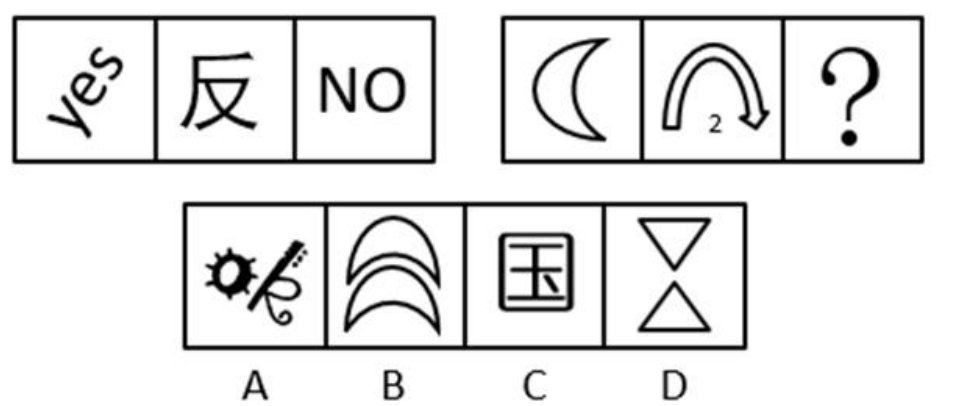
\includegraphics[scale=0.25]{40}\\ 
\end{frame}

%%%%%%%%%%%%%%%%%%%%%%%%%%%%%%%%%%%%%%%%
% A frame
%%%%%%%%%%%%%%%%%%%%%%%%%%%%%%%%%%%%%%%%
\begin{frame}[t]{推理判断(图形)}
    40\\
    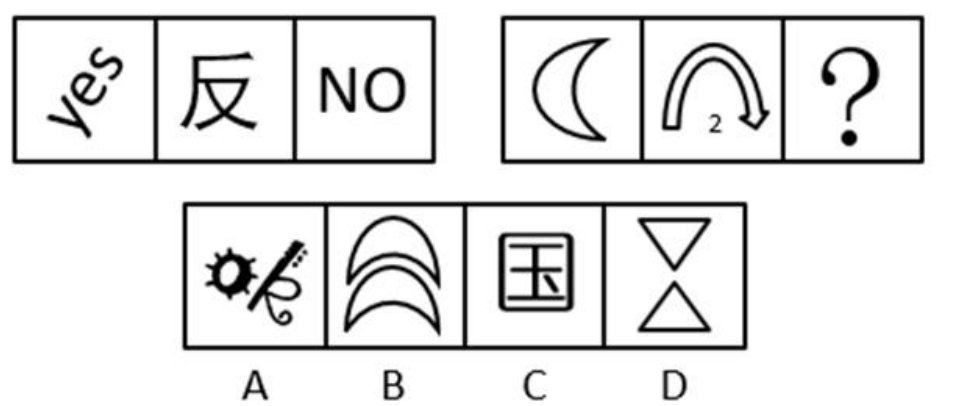
\includegraphics[scale=0.25]{40}\\ 
    解析:\textcolor{red}{C}\\
    元素组成不相同不相似,且无明显属性规律,考虑数量规律,\\
    观察提干发现出现了封闭空间,优先考虑面数量,\\
    提干中每个图形的面数量均为 1 个,故?处选择拥有 1 个面的即可.\\
    A 项 2 个,B 项 2 个,C 项 1 个,D项 2 个。\\
故正确答案为 C\\
\end{frame}


%%%%%%%%%%%%%%%%%%%%%%%%%%%%%%%%%%%%%%%%
% A frame
%%%%%%%%%%%%%%%%%%%%%%%%%%%%%%%%%%%%%%%%
\begin{frame}[t]{推理判断(图形)}
    41\\
    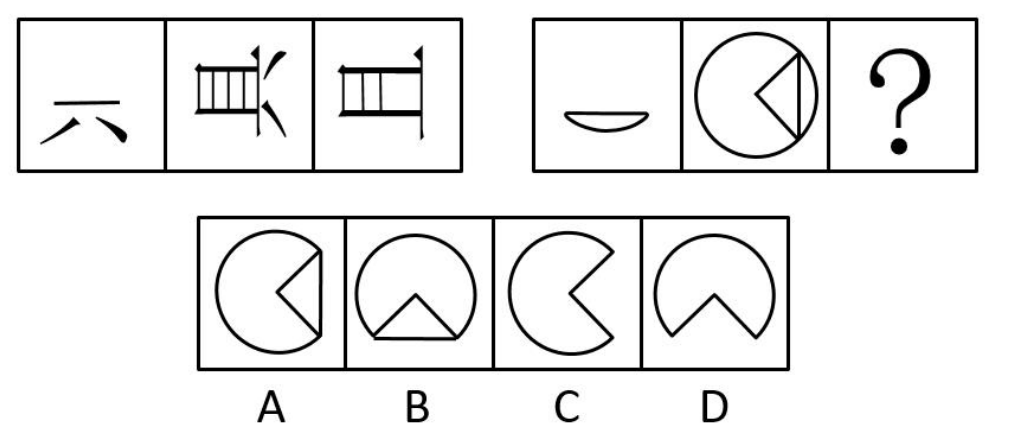
\includegraphics[scale=0.25]{41}\\ 
\end{frame}


%%%%%%%%%%%%%%%%%%%%%%%%%%%%%%%%%%%%%%%%
% A frame
%%%%%%%%%%%%%%%%%%%%%%%%%%%%%%%%%%%%%%%%
\begin{frame}[t]{推理判断(图形)}
    41\\
    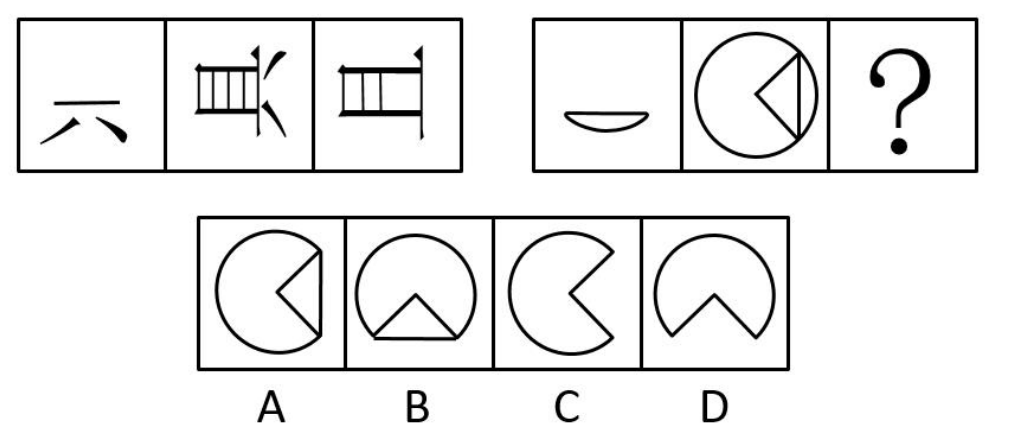
\includegraphics[scale=0.25]{41}\\ 
    解析:\textcolor{red}{C}\\
    元素组成相似,线条重复出现,考虑样式规律。\\
    再次观察第一组图形发现图 1 逆时针旋转 90 度 ,再与图 2 去同存异得到图 3,\\
    第二组图形应该遵循同样规律,只有 C 项符合要求。
故正确答案为 C
\end{frame}


%%%%%%%%%%%%%%%%%%%%%%%%%%%%%%%%%%%%%%%%
% A frame
%%%%%%%%%%%%%%%%%%%%%%%%%%%%%%%%%%%%%%%%
\begin{frame}[t]{推理判断(图形)}
    42\\
    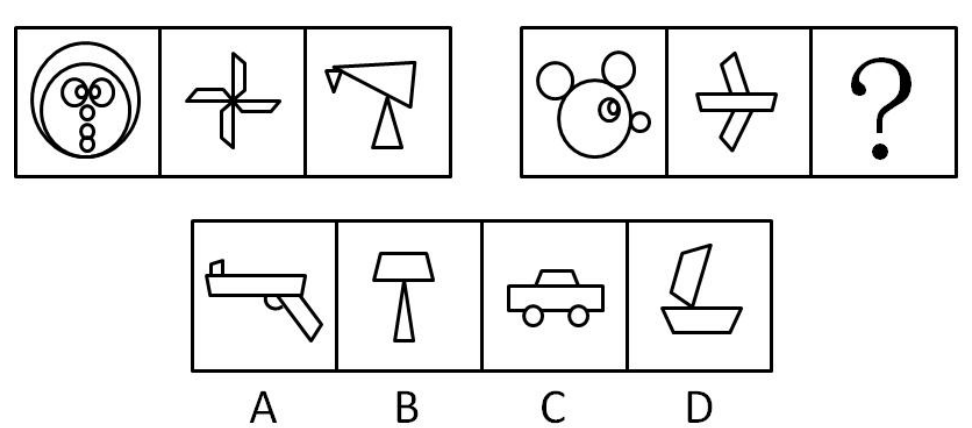
\includegraphics[scale=0.25]{42}\\ 
\end{frame}



%%%%%%%%%%%%%%%%%%%%%%%%%%%%%%%%%%%%%%%%
% A frame
%%%%%%%%%%%%%%%%%%%%%%%%%%%%%%%%%%%%%%%%
\begin{frame}[t]{推理判断(图形)}
    42\\
    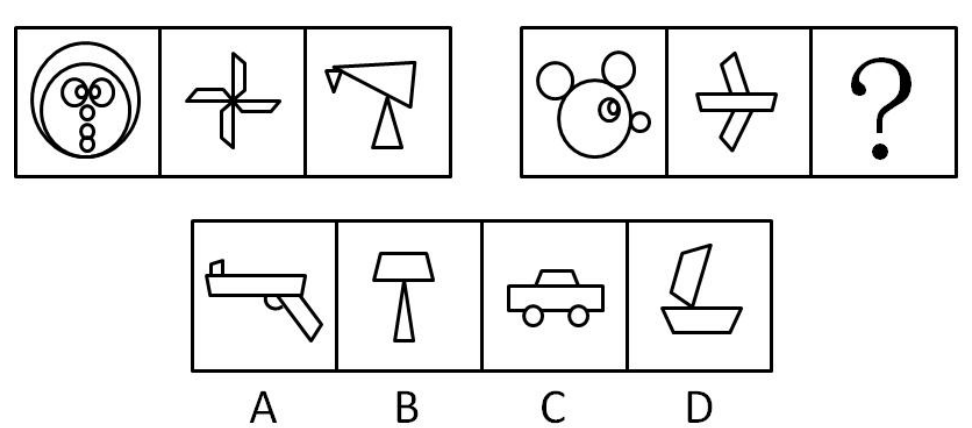
\includegraphics[scale=0.25]{42}\\ 
    解析:\textcolor{red}{D}\\
    元素组成不相同不相似,且无明显属性规律,考虑数量规律,题干中每幅图均由相同元素组成,只有
D 项符合要求。\\
故正确答案为 D\\
\end{frame}

%%%%%%%%%%%%%%%%%%%%%%%%%%%%%%%%%%%%%%%%
% A frame
%%%%%%%%%%%%%%%%%%%%%%%%%%%%%%%%%%%%%%%%
\begin{frame}[t]{推理判断(图形)}
    43\\
    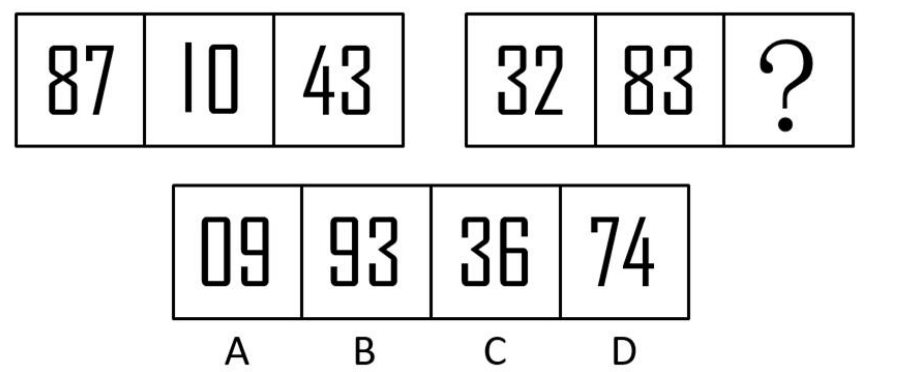
\includegraphics[scale=0.25]{43}\\ 
\end{frame}


%%%%%%%%%%%%%%%%%%%%%%%%%%%%%%%%%%%%%%%%
% A frame
%%%%%%%%%%%%%%%%%%%%%%%%%%%%%%%%%%%%%%%%
\begin{frame}[t]{推理判断(图形)}
    43\\
    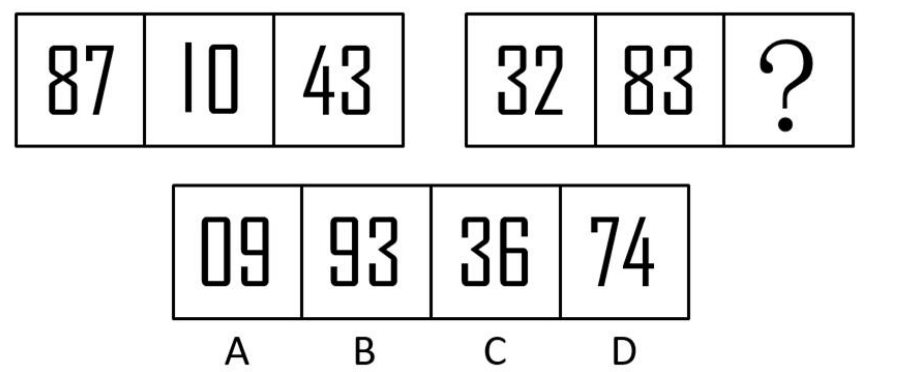
\includegraphics[scale=0.25]{43}\\ 
    解析:\textcolor{red}{D}\\
    元素组成不相同不相似,且无明显属性规律,考虑数量规律,\\
    题干中的数字出现很多端点,考虑笔画数,\\
    左侧图形笔画数分别为 2、2、3,\\
    右侧图形分别为 2、2,?\\
    ? 处应选 3 笔画图形,\\
    A 项 2 笔画,B 项 2 笔画,
    C 项 2 笔画,D 项 3 笔画,\\
    只有 D 项符合要求。\\
    故正确答案为 D\\
\end{frame}


%%%%%%%%%%%%%%%%%%%%%%%%%%%%%%%%%%%%%%%%
% A frame
%%%%%%%%%%%%%%%%%%%%%%%%%%%%%%%%%%%%%%%%
\begin{frame}[t]{推理判断(图形)}
    44\\
    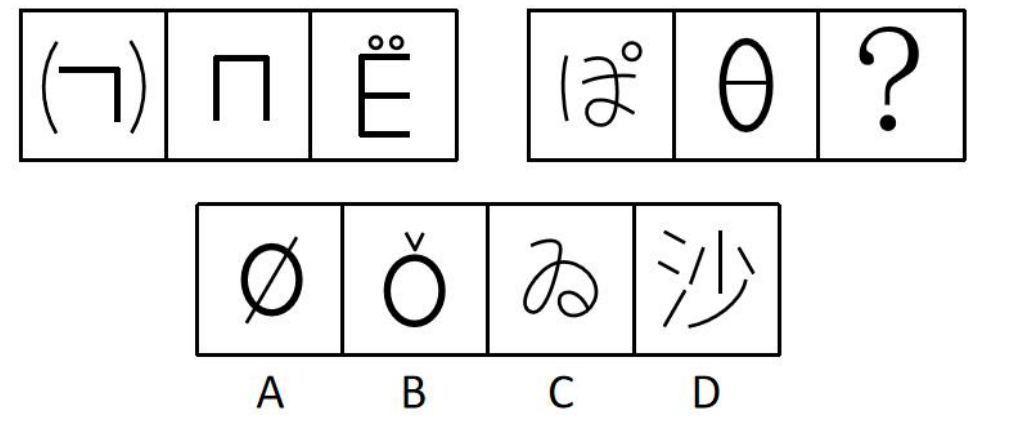
\includegraphics[scale=0.25]{44}\\ 
\end{frame}

%%%%%%%%%%%%%%%%%%%%%%%%%%%%%%%%%%%%%%%%
% A frame
%%%%%%%%%%%%%%%%%%%%%%%%%%%%%%%%%%%%%%%%
\begin{frame}[t]{推理判断(图形)}
    44\\
    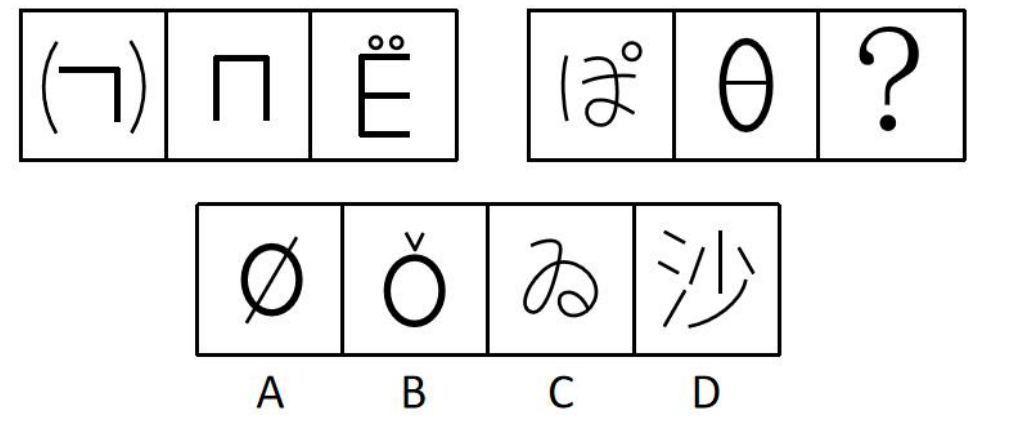
\includegraphics[scale=0.25]{44}\\ 
    解析:\textcolor{red}{B}\\
    元素组成不相同、不相似,且无明显属性规律,考虑数量规律。\\
    第一组图形,直线的数量分别是 2,3,4。\\
    第二组图,直线的数量分别为 0、1,故问号处,直线的数量应该为 2。\\
    故正确答案为 B。\\
\end{frame}





%%%%%%%%%%%%%%%%%%%%%%%%%%%%%%%%%%%%%%%%
% A frame
%%%%%%%%%%%%%%%%%%%%%%%%%%%%%%%%%%%%%%%%
\begin{frame}[t]{推理判断}
  45、有一种观点认为:人的记忆被存储在大脑皮质中,并且可以被脑电流或者外部电流所激发。这为科学幻想提供了大量素材。\\
假设上述观点为真,则( )。      \\
A、每一次输送脑电流都可以激发记忆\\
B、科学幻想都是被脑电流激发的产物\\
C、向大脑输送电流未必能将记忆激发\\
D、脑电流与外部电流的性质完全相同\\
\end{frame}


%%%%%%%%%%%%%%%%%%%%%%%%%%%%%%%%%%%%%%%%
% A frame
%%%%%%%%%%%%%%%%%%%%%%%%%%%%%%%%%%%%%%%%
\begin{frame}[t]{推理判断}
    解析:\textcolor{red}{C}\\
    根据题干信息逐一分析选项。\\
A 项:根据题干信息可知,人的记忆可以被脑电流或者外部电流所激发,但并不意味着每一次输送脑电流
都可以激发记忆,表述绝对,排除;\\
B 项:根据题干信息可知,人的记忆被激发为科学幻想提供了大量素材,但不能代表所有的科学幻想都是
被脑电流激发的产物,表述绝对,排除;\\
C 项:根据题干信息,人的记忆可以被脑电流或者外部电流激发,但是向大脑输送电流不一定能够激发人
的记忆,可以推出,当选;\\
D 项:题干并没有提及关于脑电流和外部电流性质的问题,无中生有,排除\\
\end{frame}


\begin{frame}[t]{推理判断}
46、来自东南西北的赵钱孙李四个人的职业各不相同,已知东部人是医生,西部人年龄最小而且是警察,
孙比东部人年龄大,钱是法官而且是南部人的朋友,李从未学过医。由此可知孙是( )。\\
A、南部人    \\
B、西部人    \\
C、北部人    \\
D、无法确定  \\
\end{frame}


%%%%%%%%%%%%%%%%%%%%%%%%%%%%%%%%%%%%%%%%
% A frame
%%%%%%%%%%%%%%%%%%%%%%%%%%%%%%%%%%%%%%%%
\begin{frame}[t]{推理判断}
    46、来自东南西北的赵钱孙李四个人的职业各不相同,已知东部人是医生,西部人年龄最小而且是警察,
    孙比东部人年龄大,钱是法官而且是南部人的朋友,李从未学过医。由此可知孙是( )。\\
    A、南部人    \\
    B、西部人    \\
    C、北部人    \\
    D、无法确定  \\
    解析:\textcolor{red}{A}
    由东部人是医生,西部人是警察,可知还剩下南部人和北部人。\\
    根据孙比东部人年龄大,可知孙不是东部人;\\
    结合西部人年龄最小,可得,孙也不是西部人。\\
    此时孙只能是南部人或者北部人其中的一个。
    根据钱是法官,可知钱不是东部人,也不是西部人,只能是南部人或者北部人其中的一个;
    并且钱是南部人的朋友,可知钱不是南部人,
    此时钱只能是北部人。最后剩下南部人为孙。
    故正确答案为 A
\end{frame}

\begin{frame}[t]{推理判断}
47、某工厂生产车间员工晓峰断定,所有的产品都已进行了检查,没有发现假冒伪劣产品,后经证实,晓
峰的断定为假。据此,厂长得出以下推论:\\
(1)尚未对所有的产品进行检查,但是发现了假冒伪劣产品。  \\
(2)所有的产品尚未经检查或者经检查发现了假冒伪劣产品。  \\
(3)如果对所有产品都进行检查,则可能发现假冒伪劣产品。  \\
则厂长的以上推论一定为真的是( )。                      \\
A、(1)                                                 \\
B、(2)                                                  \\
C、(1)(3)                                              \\
D、(2)(3)\\
\end{frame}


\begin{frame}[t]{推理判断}
    解析:\textcolor{red}{D}\\
    第一步:翻译题干信息。\\
    (进行检查 且 -发现假冒伪劣)为假,则它的矛盾一定为真,\\
    即:( -进行检查 或 发现假冒伪劣)为真\\

    第二步:逐一分析选项。\\
    (1)翻译为( -进行检查 且 发现假冒伪劣),题干或关系为真,\\
    不一定能得出且关系也为真,所以(1)不一定能得出;\\
    (2)翻译为: -进行检查 或 发现假冒伪劣,与题干一致,一定为真,当选;\\
    (3)翻译为:进行检查—>发现假冒伪劣,等价于: -进行检查 或 发现假冒伪\\
    因此推论一定为真的是(2)和(3)。\\
    故正确答案为 D。\\


\end{frame}






\begin{frame}[t]{推理判断}

48、文化震撼是指整个主体进入到一个非熟知的文化情境或系统后,在与之互动的过程中,所体验到的包
括精神压力在内的全部感受。根据上述定义,下列情形不属于文化震撼的是( )。\\
A、当哥伦布的船队到达美洲大陆后,船员们为当地土著迥然不同的习俗语言感到惊诧不已。             \\
B、古代某位从未听说过佛教的农民,在首次参观邻村新建成的佛教造像后,欣喜若狂。                 \\
C、大四学生魏某在出国交流半年后返校,因喜爱国外的风土人情,却又不能定居而苦恼万分。           \\
D、某乡村厨师在一线城市的一家互联网快餐店找到了一份收入可观的工作,但因无法适应建立在互联网基 
础上的快节奏工作模式而焦虑。                                                                  \\
\end{frame}

\begin{frame}[t]{推理判断}
    解析:\textcolor{red}{C}\\
    48、第一步:找出定义关键词。\\
    “进入到一个非熟知的文化情境或系统后”、\\
    “在与之互动的过程中,所体验到的包括精神压力在内的全部感受”\\
    第二步:逐一分析选项。\\
    A 项:\\
    哥伦布船队到达美洲大陆,符合“进入到一个非熟知的文化情境或系统后”,\\
    船员们为当地土著迥然不同的习俗语言感到惊诧不已,符合“在与之互动的过程中,所体验到的包括精神压力在内的全部感受”,\\
    符合定义,排除;\\
    B 项:\\
    首次参观邻村新建成的佛教造像,符合“进入到一个非熟知的文化情境或系统后”,\\
    农民感到“欣喜若狂”,符合“在与之互动的过程中,所体验到的包括精神压力在内的全部感受”,符合定义,排除;\\
\end{frame}

\begin{frame}[t]{推理判断}
    48、
    第二步:逐一分析选项。\\
    C 项:\\
    魏某在出国交流半年后,符合“进入到一个非熟知的文化情境或系统后”,\\
    但\textbf{返校后}因为不能定居而苦恼万分,是已经返回国内后的表现,不符合“与之\textbf{互动过程中},所体验到的包括精神压力在内的全部感受”,不符合定义,当选;\\
    D 项:\\
    乡村厨师进入到一线城市的互联网快餐店,符合“进入到一个非熟知的文化情境或系统后”,\\
    因无法适应建立在互联网基础上的快节奏工作模式而焦虑,符合“在与之互动的过程中,所体验到的包括精神压力
    在内的全部感受”,符合定义,排除。\\

    本题为选非题,故正确答案为 C。\\
\end{frame}






\begin{frame}[t]{推理判断}
49、告子认为人性就像柳树,仁义就像器具,柳树被外力做成器具,而不是柳树生来的样子。孟子则反驳
说,柳树被作为器具是外力暴力的破坏了树本身,事实上让人变得仁义不必像是靠外力来扭去柳树那样扭曲人
性。孟子得出结论,告子的类比是错误的。\\
孟子的结论得以成立的前提条件是( )。 \\
A、孟子的智慧远远的胜于告子           \\
B、人性本无所谓善也无所谓恶           \\
C、仁义是人生追求的崇高价值           \\
D、人性需要靠外力来产生扭转           \\
\end{frame}                           


\begin{frame}[t]{推理判断}
    解析:\textcolor{red}{C}\\
    第一步:找出论点和论据。\\
    论点:告子的类比是错误的。\\
    论据:让人变得仁义不必像是靠外力来扭去柳树那样扭曲人性\\
    论点中告子的类比指的是人性是被外力做成仁义,而不是人性生来的样子。而论据中则提到的是不必靠扭
    曲人性,可考虑建立扭曲和人性之间的关系。\\
    第二步:逐一分析选项。\\
    A 项:孟子的智慧远远胜于告子,与题干讨论的话题不一致,属于无关选项,排除;\\
    B 项:讨论的是人性善恶的问题,题干并没有提到关于善恶,属于无关项,排除;\\
    C 项,仁义是人生追求的崇高价值,说明仁义是人自发追求的,并不需要依靠外力,是论点成立的前提,
    当选。\\
    D 项,论点是人性不需要借助外力,而选项表达人性需要靠外力来产生扭转,有削弱的作用,排除。\\
    故正确答案为 C\\
\end{frame}                           


  \begin{frame}[t]{资料分析}
      50-54\\
      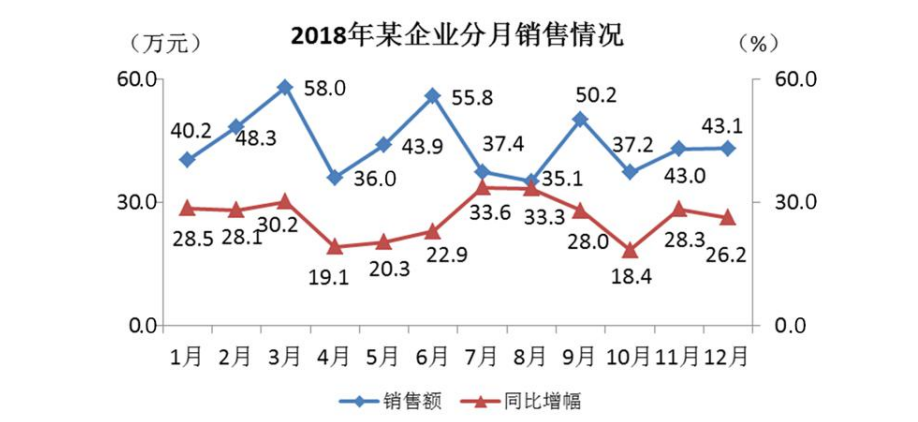
\includegraphics[scale=0.5]{50254}\\ 
  \end{frame}                           


%%%%%%%%%%%%%%%%%%%%%%%%%%%%%%%%%%%%%%%%
% A frame
%%%%%%%%%%%%%%%%%%%%%%%%%%%%%%%%%%%%%%%%
  \begin{frame}[t]{资料分析}
      50、该企业 2018 年第二季度销售额与第一季度销售额相比( )。              \\
      A、减少了 23.8 万元                                                      \\
      B、增加了 10.8 万元                                                      \\
      C、减少了 7.4\%                                                          \\ 
      D、增加了 8.0\%                                                          \\
  \end{frame}                           



%%%%%%%%%%%%%%%%%%%%%%%%%%%%%%%%%%%%%%%%
% A frame
%%%%%%%%%%%%%%%%%%%%%%%%%%%%%%%%%%%%%%%%
  \begin{frame}[t]{资料分析}
    解析:\textcolor{red}{C}\\
      根据“2018 年第二季度……与第一季度销售额相比”结合选项“增加/减少$+$ 万元”、“增加/减少\%”可判定本题为增长量计算和一般增长率问题。\\
      根据图形材料可知,2018 年 1 月-6 月销售额分别为 40.2、48.3、58.0、36.0、43.9、55.8 万元,\\
      则 2018 年第一季度销售$40.2+48.3+58=146.5$ 万元\\
      则 2018 年第二·季度销售$30.6+43.9+55.8=135.7$ 万元\\
      则\textbf{增长量 = 现期量 - 基期量}  $ = 135.7 - 146.5 =-10.8$万元\\
      即 2018 年第二季度销售额比第一季度减少 10.8 万元,排除A,B\\
      \textbf{增长率 = 增长量 / 基期量} $= \frac{-10.8}{146.5}  \approx -7.4\%$ 即减少 -7.4\%\\
      故正确答案为 C。\\

  \end{frame}                           



%%%%%%%%%%%%%%%%%%%%%%%%%%%%%%%%%%%%%%%%
% A frame
%%%%%%%%%%%%%%%%%%%%%%%%%%%%%%%%%%%%%%%%
  \begin{frame}[t]{资料分析}
      51、该企业 2018 年第 3 季度销售额较 2017 年同期增加( )万元。  \\
      A、32.9                                                         \\
      B、29.2                                                         \\
      C、23.6                                                         \\ 
      D、17.0                                                         \\
  \end{frame}                           



%%%%%%%%%%%%%%%%%%%%%%%%%%%%%%%%%%%%%%%%
% A frame
%%%%%%%%%%%%%%%%%%%%%%%%%%%%%%%%%%%%%%%%
  \begin{frame}[t]{资料分析}
    解析:\textcolor{red}{B}\\
    根据“2018 年第 3 季度……较 2017 年同期万元 增加……万元”,可判定本题为增长量计算问题。\\
    总体增量 = 部分增量之和,2018 年第 3 季度同比增量 = 2018 年7月同比增量 + 2018 年8月同比增量  + 2018 年9月同比增量 \\
    2018年 7 到 9  月销售额分别为 37.4、35.1、50.2 万元, 同比增速分别为 33.6\%, 33.3\%, 28.0\% \\

      代入公式 增长量 = (现期/ $1+r$)$\times  r$ \\

      2018 年 7 月销售额同比增量 $=  \frac{37.4}{1+33.6\%} \times 33.6\% \approx  \frac{37.4}{1+\frac{1}{3}} \times \frac{1}{3} \approx \frac{37.4}{4} \approx 9.4 $ 万元\\
      2018 年 8 月销售额同比增量 $=  \frac{35.1}{1+33.3\%} \times 33.3\% \approx  \frac{35.1}{1+\frac{1}{3}} \times \frac{1}{3} \approx \frac{35.1}{4} \approx 8.8 $ 万元\\
      2018 年 9 月销售额同比增量 $=  \frac{50.2}{1+28.0\%} \times 28.0\% \approx  \frac{50.2}{1+\frac{1}{3.5}} \times \frac{1}{3.5} \approx \frac{50.2}{4} \approx 11.2 $ 万元\\
      则 2018 年第 3 季度销售额同比增量约为$9.4+8.8+11.2=29.4$ ,与 B 选项最接近。故正确答案为 B\\
  \end{frame}                           





%%%%%%%%%%%%%%%%%%%%%%%%%%%%%%%%%%%%%%%%
% A frame
%%%%%%%%%%%%%%%%%%%%%%%%%%%%%%%%%%%%%%%%
  \begin{frame}[t]{资料分析}
      52、该企业 2018 年 1-12 月当月销售额未达到全年平均月销售额的月份有( )个。  \\
      A、4                                                                         \\
      B、5                                                                         \\
      C、7                                                                         \\ 
      D、8                                                                         \\
  \end{frame}                           


%%%%%%%%%%%%%%%%%%%%%%%%%%%%%%%%%%%%%%%%
% A frame
%%%%%%%%%%%%%%%%%%%%%%%%%%%%%%%%%%%%%%%%
  \begin{frame}[t]{资料分析}
    解析:\textcolor{red}{D}\\
    由题干“2018 年 1-12 月当月……未达到全年平均月……有( )个”,可判定该题为现期平均数。
    { \scriptsize
    \begin{gather}
        \text{2018全年销售额} = \frac{\text{总销售额}}{\text{月份数}} \\
        = \frac{40.2 + 48.3 + 58.0 + 36.0 + 43.9 + 55.8+ 37.4 + 35.1+50.2+37.2+43.0+43.1}{12} \\
        = \frac{12 \times 44 + (-3.8+4.3+14-8-0.1+11.8-6.6-8.9+6.2-6.8-1-0.9)}{12} \\
        = \frac{12 \times 44 + 0.2}{12} \\
        \approx 44
    \end{gather}
    }

      则未达到全年
平均水平,即 1-12 月各月份销售额低于 44 的有 1 月、4 月、5 月、7 月、8 月、10 月、11 月、12 月共 8 个月。\\
故正确答案为 D
  \end{frame}                           





%%%%%%%%%%%%%%%%%%%%%%%%%%%%%%%%%%%%%%%%
% A frame
%%%%%%%%%%%%%%%%%%%%%%%%%%%%%%%%%%%%%%%%
  \begin{frame}[t]{资料分析}
      53、该企业 2018 年第一季度各月销售额同比增长最多的月份是( )。  \\
      A、3 月                                                          \\
      B、2 月                                                          \\
      C、1 月                                                          \\ 
      D、无法判断                                                      \\
  \end{frame}                           

%%%%%%%%%%%%%%%%%%%%%%%%%%%%%%%%%%%%%%%%
% A frame
%%%%%%%%%%%%%%%%%%%%%%%%%%%%%%%%%%%%%%%%
  \begin{frame}[t]{资料分析}
      解析:\textcolor{red}{A}\\
      根据“2018 年第一季度各月……增长最多的月份是”,可判定本题为增长量比较问题。\\
      定位图形材料可知,2018 年第一季度,即 1、2、3 月销售额分别为 40.2、48.3、58.0 万元,增长率分别为 28.5\%, 28.1\%, 30.2\%。\\
      根据增长量比较口诀“大大则大”可知,2018 年 3 月现期最大(58.0),增长率最大(30\% ),则其增长量一定最大。\\
      即 2018 年 3 月销售额同比增长最多。\\
      故正确答案为 A
  \end{frame}                           

%%%%%%%%%%%%%%%%%%%%%%%%%%%%%%%%%%%%%%%%
% A frame
%%%%%%%%%%%%%%%%%%%%%%%%%%%%%%%%%%%%%%%%
  \begin{frame}[t]{资料分析}
      54、根据上图,以下说法不正确的是( )。                         \\
      A、2018 年第一季度,该企业的销售额月均增长率不超过 15\%         \\
      B、2018 年 1-4 季度,第三季度月平均销售额最低                   \\
      C、2018 年 2-12 月当月销售额环比降幅最大的月份是 4 月           \\ 
      D、2018 年 1-4 季度各季度销售额最高的月份都是该季度最后一个月   \\
  \end{frame}                           

%%%%%%%%%%%%%%%%%%%%%%%%%%%%%%%%%%%%%%%%
% A frame
%%%%%%%%%%%%%%%%%%%%%%%%%%%%%%%%%%%%%%%%

  \begin{frame}[t]{资料分析}
      解析:\textcolor{red}{A}\\
      A 项:2018 年第一季度销售额月均增长率,即 2018 年 1-3 月月均增长率。\\
      定位图形数据可知,2018 年 1月销售额为 40.2 万元,3 月销售额为 58.0 万元。\\
      根据年均增长率(月均增长率)公式:\\
      { \tiny
      \begin{gather}
          (1+r)^n = \frac{\text{现期}}{\text{基期}}
      \end{gather}
      }
      { \tiny
      \begin{gather}
          (1+r)^n = \frac{\text{现期}}{\text{基期}} = \frac{58}{40.2} \approx 1.44
      \end{gather}
      }
      { \tiny
      \begin{gather}
          1+r \approx 1.2
      \end{gather}
      }
      { \tiny
      \begin{gather}
          r \approx 0.2  = 20\% 
      \end{gather}
      }
      超过 15\% ,错误。
  \end{frame}                           

%%%%%%%%%%%%%%%%%%%%%%%%%%%%%%%%%%%%%%%%
% A frame
%%%%%%%%%%%%%%%%%%%%%%%%%%%%%%%%%%%%%%%%
  \begin{frame}[t]{资料分析}
      解析:\textcolor{red}{A}\\
      B 项:由于每个季度均有 3 个月,因此比较各季度平均销售额可直接比较各季度总销售额。\\
      根据图形数据可知 2018 年 1-12 月各月的销售额: 
      $\text{2018年1季度销售额 }= 1 \text{月} + 2 \text{月}  + 3 \text{月}   = 40.2 + 48.3 +58.0 = 146.5     $
      $\text{2018年2季度销售额 }= 4 \text{月} + 5 \text{月}  + 6 \text{月}   = 36.0 + 43.9 +55.8 = 135.7     $
      $\text{2018年3季度销售额 }= 7 \text{月} + 8 \text{月}  + 9 \text{月}   = 37.4 + 35.1 +50.2 = 122.7     $
      $\text{2018年4季度销售额 }= 10 \text{月} + 11 \text{月}  + 12 \text{月}   = 37.2 + 43.0 +43.1 = 123.3  $\\
      第 3 季度总销售额最低,则第 3 季度月平均销售额也最低,正确;\\
  \end{frame}                           
%%%%%%%%%%%%%%%%%%%%%%%%%%%%%%%%%%%%%%%%
% A frame
%%%%%%%%%%%%%%%%%%%%%%%%%%%%%%%%%%%%%%%%
  \begin{frame}[t]{资料分析}
      解析:\textcolor{red}{A}\\
      C 项:定位图形数据可知 2018 年 2-12 月各月的销售额,出现环比下降的有 4 月、7 月、8 月、10 月。根据
      公 式 $\text{增长率} = \frac{\text{现期量} - \text{基期量}}{\text{基期量}}$
      $\text{2018年4月环比增长率} = \frac{36-58}{58} = \frac{-22}{58} \approx -38\%$
      $\text{2018年7月环比增长率} = \frac{37.4-55.8}{55.8} = \frac{-18.4}{55.8} \approx -33\%$
      $\text{2018年8月环比增长率} = \frac{35.1-37.4}{37.4} = \frac{-2.3}{37.4} \approx -6\%$
      $\text{2018年10月环比增长率} = \frac{37.2-50.2}{50.2} = \frac{-13}{50.2} \approx -26\%$
      环比降幅最大为 4 月,正确\\
      D 项:\\
      定位图形数据可知,2018 年 1-4 季度各季度销售额最高的月份分别是 3 月、6 月、9 月、12 月,确
      实都是季度的最后一个月,正确;\\
      本题为选非题,故正确答案为 A。 \\
  \end{frame}                           

  

  \begin{frame}[t]{资料分析}
      55-59\\
      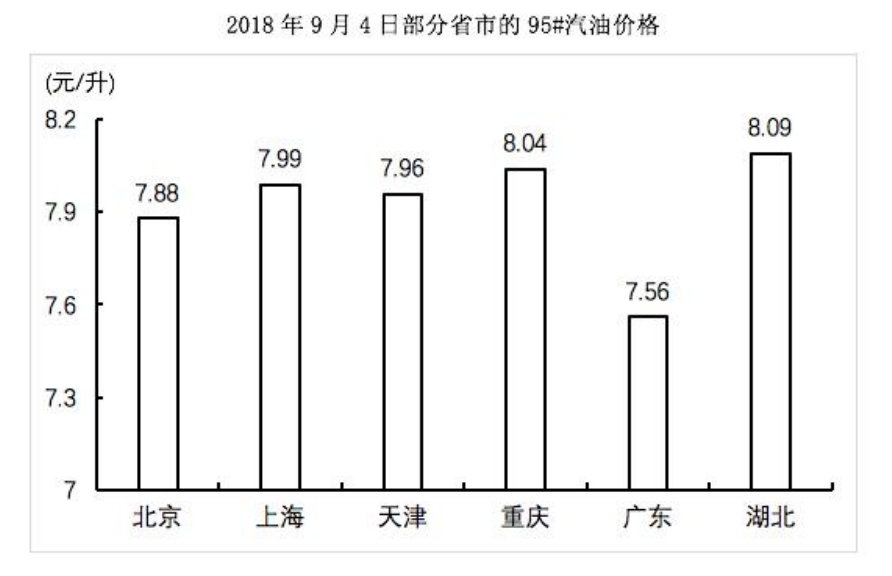
\includegraphics[scale=0.29]{55259-1}
      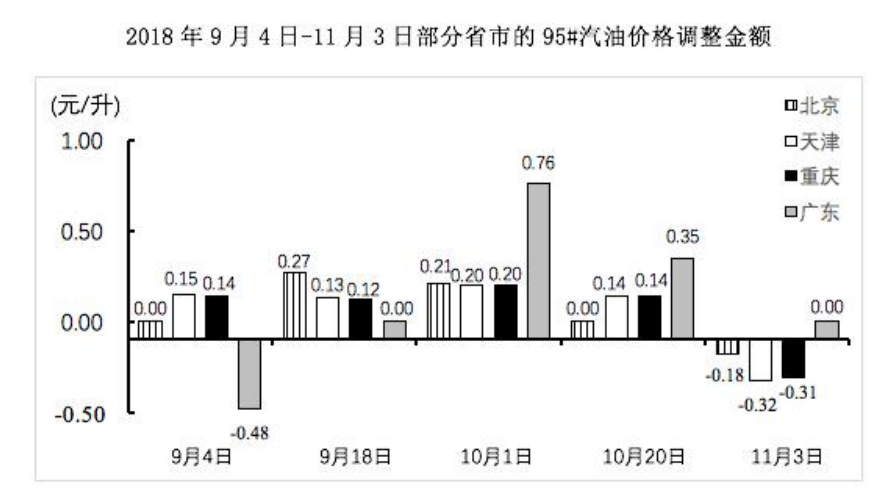
\includegraphics[scale=0.29]{55259-2}
  \end{frame}                           


  \begin{frame}[t]{资料分析}
      55、北京,天津,重庆,广东 4 个省市中,11 月 3 日的 95\# 汽油价格与 9 月 4 日相比,变化最大与变化量
      最小的省市之间,变化量相差( )元/升。\\
      A、0.34                               \\
      B、0.75                               \\
      C、0.96                               \\
      D、1.21                               \\
  \end{frame}                           

  \begin{frame}[t]{资料分析}
      55、\textcolor{red}{C}\\
      {\small
      定位图二,可知 9 月 4 日至 11 月 3 日北京、天津、重庆、广东的 95\#汽油价格调整金额。\\
      11 月 3 日95\#汽油价格较 9 月 4 日的变化量,\\
      等于 9 月 18 日至 11 月 3 日 4 次调整金额之和的绝对值\\
      \begin{gather}
          \text{北京:} 0.27+0.21+0.00+(-0.81) = 0.30 \text{元/升}\\
          \text{天津:} 0.13+0.20+0.14+(-0.32) = 0.15 \text{元/升}\\
          \text{重庆:} 0.12+0.20+0.14+(-0.31) = 0.15 \text{元/升}\\
          \text{广东:} 0.00+0.76+0.35+0.00 = 1.11 \text{元/升}
      \end{gather}
      则变化量最大的省份为广东(1.11 元/升),最小的省份为天津和重庆(均为 0.15 元/升)\\
      变化差值$=1.11 - 0.15 = 0.96$ 元/升\\
      }
  \end{frame}                           


  \begin{frame}[t]{资料分析}
      56、某公司每天均在广东省内加 30 升 95\#汽油,从 9 月 3 日到 9 月 30 日共需油费( )元。\\
      A、241.2                                                                              \\
      B、6350.4                                                                             \\
      C、6123.6                                                                             \\
      D、6364.8                                                                             \\
  \end{frame}                           

  \begin{frame}[t]{资料分析}
      56、\\
      定位图一可知 9 月 4 日广东省95\# 汽油价格为 7.56 元/升,\\
      定位图二可知 9 月 4 日汽油价格下调 0.48元/升,9 月 18 日汽油价格未发生调整。\\
      9 月 3 日汽油价格$=7.56+0.48=8.04$  元/升,当日加 30 升汽油花费 $8.04 \times 30=241.2 元$;\\
      因 9 月 18 日汽油价格未发生调整,所以 9 月 4 日至 9 月 30 日汽油价格保持 7.56 元/升 不 变 ,
      该 时 期 加 30 升 汽 油 花 费 $7.56 \times 30 \times 27 = 6123.6$。\\
      9 月 3 日 至 9 月 30 日 共 花 费 $241.2 +6123.6 =6364.8$ 元。\\
      因本题为精确计算,且选项尾数不同,所以也可采用尾数法来做,总的油费为 $8.04 \times 30 + 7.56 \times 30 \times 27$
      ,式子前面尾数为 0.2,式子后面尾数为 0.6,所以式子的尾数为$0.2+0.6 = 0.8$ ,满足
      的只有 D 选项。\\
      故正确答案为 D。
  \end{frame}                           










  \begin{frame}[t]{资料分析}
      57、若 9 月 4 日上海,湖北的 95\#汽油价格分别上调 0.13 元/升,0.14 元/升,则这 6 个省市中,9 月 4 日
      汽油价格增幅最大的是( )。\\
      A、上海                    \\
      B、天津                    \\
      C、湖北                    \\
      D、广东                    \\
  \end{frame}                           


  \begin{frame}[t]{资料分析}
      57、根据题干“……增幅最大的是”,可判定本题为增长率的比较问题。\\
      只需计算选项中的 4 个城市,定位图一可知 9 月 4 日上海、天津、广东、湖北 95\#汽油价格分别为 7.99 元/升、7.96 元/升、7.56 元/升、8.09
      元/升,\\
      定位图二可知 9 月 4 日天津汽油价格上调 0.15 元/升,广东下调 0.48 元/升,\\
      根据题干已知 9 月 4 日上海、湖北的 汽油价格分别上调 0.13 元/升、0.14 元/升。根据公式:
      $\text{增长率} = \frac{\text{增长量} - \text{现期量}}{\text{增长量}}$
      ,则 9 月 4日汽油价格增幅如下,
      \begin{gather}
          \text{上海:} \frac{0.13}{7.99-0.13} = \frac{0.13}{7.86}\\
          \text{天津:}\frac{0.15}{7.96-0.15} = \frac{0.15}{7.81}\\
          \text{湖北:}\frac{0.14}{8.09-0.14} = \frac{0.14}{7.95}
      \end{gather}
      广东汽油价格下调,增长率为负,排除。\\
      前三个式子中,明显天津的增幅分子最大且分母最小,\\
      故 9 月 4 日 汽油价格增幅最大的是天津。故正确答案为 B\\
  \end{frame}                           


  \begin{frame}[t]{资料分析}

      58、若上一轮的全国油价调整时间为 8 月 25 日,则以下时间段内,北京市 95\#汽油价格不变天数最多的是( )。          \\
      A、8 月 16 日-9 月 9 日                                                                                         \\
      B、9 月 18 日-10 月 2 日                                                                                        \\
      C、10 月 20 日-11 月 3 日                                                                                       \\
      D、11 月 1 日-11 月 15 日                                                                                       \\

  \end{frame}                           


  \begin{frame}[t]{资料分析}
      58、定位图二可知 9 月 4 日至 11 月 3 日北京市95\# 汽油价格调整金额,题干给出上一轮的全国油价调整时
      间为 8 月 25 日,根据所给数据逐个分析选项:\\

      A 项,8 月 16 日至 9 月 9 日期间,因 9 月 4 日价格未调整,则价格保持不变天数最多的是 8 月 25 日至 9
      月 9 日共 16 天。8 月 16 日至 8 月 24 日情况未知,所以该期间至少有 \textbf{16} 天保持不变;\\

      B 项,9 月 18 日至 10 月 2 日期间,因 10 月 1 日价格上调,则价格保持不变的天数最多的是 9 月 18 日至 9
      月 30 日共 \textbf{13} 天;\\

      C 项,10 月 20 日至 11 月 3 日期间,因 11 月 3 日价格下调,则价格保持不变天数最多的是 10 月 20 日至
      11 月 2 日共 \textbf{14} 天;\\

      D 项,11 月 1 日至 11 月 15 日期间,因 11 月 3 日价格下调且下次调整时间未知,故价格保持不变天数最多
      的是 11 月 3 日至 11 月 15 日,所以该期间至多 \textbf{13} 天保持不变。\\

      综上所述,A 项 8 月 16 日至 9 月 9 日期间保持不变天数最多。故正确答案为 \textcolor{red}{A}\\

  \end{frame}                           









  \begin{frame}[t]{资料分析}
      59、根据上图,以下说法错误的是( )。                                          \\
      A、9 月 19 日,北京,天津,重庆,广东四个省市中,95\#汽油价格最高的是重庆       \\
      B、9 月 4 日-11 月 3 日进行的五次油价调整中,北京和广东均有两次未发生价格变动  \\
      C、9 月 4 日-11 月 3 日,天津和重庆的 95\#汽油价格变化趋势相同                  \\
      D、9 月 4 日四个直辖市的 95\#汽油平均价格是 8.07 元/升                          \\
  \end{frame}                           


  \begin{frame}[t]{资料分析}
      59、解析:\textcolor{red}{D}\\
      {\scriptsize
      A 项:定位图一可知 9 月 4 日,北京、天津、重庆、广东四个省市 95\#汽油价格分别为 7.88 元/升、7.96元/升、8.04 元/升、7.56 元/升,\\
      定位图二可知 9 月 18 日北京、天津、重庆、广东四个省市95\# 汽油调整金额分 别 为 0.27 元 / 升 、 0.13 元 / 升 、 0.12 元 / 升 、 0.00 元 / 升 。 \\
      则 9 月 19 日\\
      北京 95\#汽油价格 $7.88+0.27=8.15$ 元/升,\\
      天津 95\#汽油价格 $7.96+0.13=8.09$ 元/升,\\
      重庆 95\#汽油价格 $8.04+0.12=8.16$ 元/升,\\
      广东 95\#汽油价格 $7.56+0.00=7.56$ 元/升,\\
      重庆 汽油价格最高,正确;\\
      B 项:定位图二可知,9 月 4 日至 11 月 3 日进行的五次油价调整中,北京在 9 月 4 日和 10 月 20 日未发生
      价格变动,广东在 9 月 18 日和 11 月 3 日未发生价格变动,均有两次,正确;\\
      C 项:定位图二可知,9 月 4 日至 11 月 3 日,天津和重庆的95\# 汽油价格均保持先升后降的趋势,正确;\\
      D 项:定位图一可知,9 月 4 日四个直辖市(北京、上海、天津、重庆) 汽油价格分别为 7.88 元/升、
      7.99 元/升、7.96 元/升、8.04 元/升, $\text{平均价格} = \frac{\text{价格总数}}{\text{城市个数}}  =  \frac{7.88 + 7.99 + 7.96 + 8.04}{4} = \frac{31.87}{4}= \frac{32}{4}  = 8$  元/升、
      即 95\#汽油平均价格不足 8 元/升,并非 8.07 元/升,错误。
      本题为选非题,故正确答案为 D。
      }
  \end{frame}                           

%%%%%%%%%%%%%%%%%%%%%%%%%%%%%%%%%%%%%%%%%%%%%%%%%%%%%%%%%%%%%%%%%%%%%%%%%%%%%%%%%%%%%%%%%%%%%%%%%%%%%%%%%%%%%%%%%%%%%%%%
  \end{comment}







  \begin{frame}[t]{资料分析}
      60-64\\
      {\scriptsize
      与 2017 年上半年相比,2018 年上半年国内旅游人数中,城镇居民 19.97 亿人次,增长 13.7\%;农村居民8.29 亿人次,增长 6.3\%。国内旅游收入中,城镇居民花费 1.95 万亿元,增长 13.7\%;农村居民花费 0.50 万亿元,增长 8.3\%,入出境旅游总数 1.41 亿人次,同比增长 6.9\%。国际旅游收入 617 亿美元,比上年同期增长 2.8\%。其中:外国人在华花费 354 亿美元,增长 4.6\%;\\

      香港同胞在内地花费 142 亿美元,下降 2.5\%;\\
      澳门同胞在内地花费 42 亿美元,增长 4.2\%;\\
      台湾同胞在大陆花费 79 亿美元,增长 4.2\%;\\
      入境旅游人数 6923 万人次,比上年同期下降 0.4\%。\\
      其中:外国人 1482 万人次,增长 4.0\%;\\
      香港同胞 3908 万人次,下降 2.7\%;
      澳门同胞 1233 万人次,增长 1.1\%;
      台湾同胞 300 万人次,增长 4.1\%。
      入境旅游人数按照入境方式分,船舶占 3.3\%,飞机占 17.1\%,火车占 0.8\%,汽车占 22.5\%,其余为徒步方式。\\
      入境过夜旅游人数 3073 万人次,其中:外国人 1144 万人次,增长 4.4\%;\\
      香港同胞 1388 万人次,下降 0.8\%;
      澳门同胞 271 万人次,增长 4.9\%;
      台湾同胞 270 万人次,增长4.1\%。
      上半年,我国主要客源市场前 17 位国家如下:缅甸、越南、韩国、日本、美国、俄罗斯、蒙古、马来西
      亚、菲律宾、新加坡、加拿大、印度、泰国、澳大利亚、印度尼西亚、德国、英国。

      }
  \end{frame}                           



  \begin{frame}[t]{资料分析}
      60、2018 年上半年,我国居民国内旅游每人次平均花费约( )元。   \\
      A、867                                                         \\
      B、881                                                         \\
      C、893                                                         \\
      D、905                                                         \\
  \end{frame}                           


  \begin{frame}[t]{资料分析}
      根据题干“2018 年上半年,……每人次平均花费”,可判定本题为现期平均数问题。\\
      定位文字材料可得:
      2018 年上半年国内旅游人数中,\\
      城镇居民 19.97 亿人次,农村居民 8.29 亿人次;\\
      国内旅游收入中,\\
      城镇居民花费 1.95 万亿元,农村居民花费 0.50 万亿元。\\
      根据公式:$\text{平均数} = \frac{\text{总数}}{\text{个数}}$ ,可得:2018 年上半年,
      {\small
      \begin{gather}
          \text{我国居民国内旅游每人平均花费}   =  \frac{\text{总花费}}{\text{总人次}}\\
                                                =  \frac{1.95+0.50}{19.95 +8.29}
                                                =  \frac{2.45\text{万亿元}}{28.26\text{亿人次}}
                                                =  \frac{24500\text{元}}{28.26\text{人次}}
                                                \approx  \frac{24500\text{元}}{28.3\text{人次}}
                                                \approx  \frac{866\text{元}}{\text{人次}}
      \end{gather}
      }
      与 A项最接近。
      故正确答案为 A\\
  \end{frame}                           





  \begin{frame}[t]{资料分析}
      61、2017 年上半年,港澳台同胞在内地花费金额约( )亿美元。\\
      A、205                                                    \\
      B、218                                                    \\
      C、221                                                    \\
      D、262                                                    \\
  \end{frame}                           



  \begin{frame}[t]{资料分析}
      62、2018 年上半年,以徒步方式入境旅游的人数约( )万人次。\\
      A、3075                                                   \\
      B、3279                                                   \\
      C、3451                                                   \\
      D、3898                                                   \\
  \end{frame}                           



  \begin{frame}[t]{资料分析}
      63、2018 年上半年,下列人员按入境过夜旅游人数由多至少排列,依次是( )。 \\
      A、香港同胞>外国人>澳门同胞>台湾同胞                                  \\
      B、香港同胞>外国人>台湾同胞>澳门同胞                                  \\
      C、外国人>香港同胞>澳门同胞>台湾同胞                                  \\
      D、外国人>香港同胞>台湾同胞>澳门同胞                                  \\
  \end{frame}                           


  \begin{frame}[t]{资料分析}
      64、根据上文,以下说法错误的是( )。                                         \\
      A、2018 年上半年,由于香港同胞入境旅游人数同比下降,导致入境旅游人数同比下降  \\
      B、2018 年上半年,入境过夜旅游人数同比呈增长趋势                              \\
      C、2018 年上半年,入境旅游平均每人次花费金额同比增长 3.2\%                    \\
      D、2018 年上半年,国际旅游收入同比增长超过 30 亿美                            \\
  \end{frame}                           



  \begin{frame}[t]{资料分析}
      61、根据题干“2017 年上半年,港澳台同胞在内地花费金额”,结合材料时间是 2018 年上半年,可判定
      本题为基期计算问题。\\
      定位文字材料可得:香港同胞在内地花费 142 亿美元,下降 2.5\%;\\
      澳门同胞在内地花费42 亿美元,增长 4.2\%;\\
      台湾同胞在大陆花费 79 亿美元,增长 4.2\%。\\
      根据公式:$\text{基期量} = \frac{\text{现期量}}{\text{1+增长率}}$ ,可得:\\
      2017年上半年港澳台同胞在内地花费金额
      \begin{gather}
          = \frac{142}{1-2.5\%} + \frac{42}{1+4.2\%} + \frac{79}{1+4.2\%} 
          = \frac{142}{1-2.5\%} + \frac{142}{1+4.2\%} 
          \approx 
      \end{gather}
      ,与 D 选项最接近。
      故正确答案为 D
  \end{frame}                           






%%%%%%%%%%%%%%%%%%%%%%%%%%%%%%%%%%%%%%%%%%%%%%%%%%%%%%%%%%%%%%%%%%%%%%%%%%%%%%%%%%%%%%%%%%%%%%%%%%%%%%%%%%%%%%%%%%%%%%%%
  \begin{comment}

  \begin{frame}[t]{综合知识}
      70、习近平总书记在第二届“一带一路”国际合作高峰论坛开幕式上强调:“我们要秉持共商共建共享原
      则,倡导多边主义······通过双边合作、三方合作、多边合作等各种形式,把大家的优势和潜能充分发
      挥出来,聚沙成塔、积水成渊”。上述讲话用典主要体现的哲学理论是( )。    \\
      A、事物的发展是前进性和曲折性的统一                                     \\
      B、量变是质变的必要前提                                                 \\
      C、发展的实质是新事物的产生与旧事物的灭亡                               \\
      D、任何真理都有其适用的条件和范围                                       \\
  \end{frame}                           


  \begin{frame}[t]{综合知识}
      70、解析:\textcolor{red}{B}\\
      本题考查政治常识。\\
      A 项错误,唯物辩证法认为,事物发展的前途是光明的,道路是曲折的。任何事物的发展都是前进性与曲
      折性的统一。题干并没有体现该哲学理论。\\
      B 项正确,量变是质变的必要前提,质变是量变的必然结果。多种形式的“合作”是量的积累,各国把优
      势和潜能充分发挥出来,“聚沙成塔、积水成渊”,到一定程度就会推动国家的发展。\\
      C 项错误,发展的实质是新事物的产生和旧事物的灭亡。新事物之所以“新”,其根本原因在于新事物符
      合客观规律。题干未提及发展的观点。\\
      D 项错误,“任何真理都有自己适用的范围和条件”,是指真理具有相对性。题干未提及真理的观点。\\
      故正确答案为 B
  \end{frame}                           


  \begin{frame}[t]{综合知识}
      71、根据《中国共产党党员教育管理工作条例》,党员教育管理的首要政治任务是( )。  \\
      A、引导党员掌握并自觉运用马克思主义立场观点方法                                  \\
      B、教育党员不忘初心牢记使命                                                      \\
      C、用习近平新时代中国特色社会主义思想武装全党                                    \\
      D、在全党范围内造成既有民主又有集中,既有自由又有纪律的政治局面                  \\
  \end{frame}                           

  \begin{frame}[t]{综合知识}
      71、解析:\textcolor{red}{C}\\
      本题考查政治常识。
《中国共产党党员教育管理工作条例》第五条指出:“把用习近平新时代中国特色社会主义思想武装全党
作为党员教育管理的首要政治任务,引导党员充分认识学习贯彻习近平新时代中国特色社会主义思想的重大意
义,自觉学懂弄通做实。”\\
故正确答案为 C
  \end{frame}                           



  \begin{frame}[t]{综合知识}
      72、香港特别行政区按照《中华人民共和国香港特别行政区基本法》(简称《基本法》)的规定实行高度
      自治,关于其立法方面的制度,下列说法错误的是( )。   \\
      A、其立法机关制定的任何法律均不得同《基本法》相抵触   \\
      B、其立法机关制定的法律报全国人大常委会批准后生效     \\
      C、全国人大常委会可将不符合《基本法》的有关法律发回   \\
      D、立法机关可使用中、英双语立法                       \\
  \end{frame}                           


  \begin{frame}[t]{综合知识}
      72、解析:\textcolor{red}{B}\\
      本题考查法律常识。\\
      { \small

      A 项正确,根据《香港特别行政区基本法》第十一条第二款规定:“香港特别行政区立法机关制定的任何
      法律,均不得同本法相抵触。”\\

      B 项错误,《香港特别行政区基本法》第十七条第两款规定:“香港特别行政区的立法机关制定的法律须
      报全国人民代表大会常务委员会备案。备案不影响该法律的生效。”其立法机关制定的法律生效不以全国人民
      代表大会常务委员会批准为前提。\\

      C 项正确,《中华人民共和国香港特别行政区基本法》第十七条第三款规定:“全国人民代表大会常务委
      员会在征询其所属的香港特别行政区基本法委员会后,如认为香港特别行政区立法机关制定的任何法律不符合
      本法关于中央管理的事务及中央和香港特别行政区的关系的条款,可将有关法律发回,但不作修改。经全国人
      民代表大会常务委员会发回的法律立即失效。”\\

      D 项正确,《中华人民共和国香港特别行政区基本法》第九条规定:“香港特别行政区的行政机关、立法
      机关和司法机关,除使用中文外,还可使用英文,英文也是正式语言。”\\

      本题为选非题,故正确答案为 B\\

      }
  \end{frame}                           


  \begin{frame}[t]{综合知识}
      73、一个行政组织的事权按照横向的水平分工,交由若干平行的部门或单位分别处理与行使,且每一个部
      门或单位所管辖的事权在性质上是部分的,在领域上是完整的。这种行政组织体制称为( )。 \\
      A、分权制                                                                           \\
      B、分级制                                                                           \\
      C、分职制                                                                           \\
      D、分离制                                                                           \\
  \end{frame}                           



  \begin{frame}[t]{综合知识}
      73、解析:\textcolor{red}{C}\\
      A 项错误,分权制是指行政决策权由上下级机关合理划分,下级机关在其权力范围内可以自主处理政务的
      行政领导体制。\\
      B 项错误,分级制是指行政组织纵向分为若干层次,上下层业务性质相同,但有隶属关系,业务范围由上
      至下逐层缩小的组织体制。\\
      C 项正确,分职制是一个行政组织的事权按照横向的水平分工,交由若干平行的部门或单位分别处理与行
      使,且每一个部门或单位所管辖的事权在性质上是部分的,在领域上是完整的。\\
      D 项错误,分离制是指同一层次各行政组织或同一行政组织各机构分属两个以上平行的或双重的上级组织
      或首长的指挥或控制,或者其中有些组织或机构具有很大的独立性,不受或很少受上级组织或首长的指挥和控
      制的组织体制。\\
      故正确答案为 C\\
  \end{frame}                           






  \begin{frame}[t]{综合知识}
      74、川滇藏印道是古代中国西南地区与南亚地区的一条著名商贸通道,因其所主要运输的物品而又被称为
      ( )。          \\
      A、万里茶道      \\
      B、仓米古道      \\
      C、川盐古道      \\
      D、茶马古道      \\
  \end{frame}                           

  \begin{frame}[t]{综合知识}
      74、解析:\textcolor{red}{D}\\
      {\small
      本题考查人文常识。\\
      A 项错误,万里茶道是继丝绸之路衰落之后在欧亚大陆兴起的又一条重要的国际商道,自中国南部产茶区
      向北穿越蒙古,到达中俄边境通商口岸恰克图并延伸至莫斯科,是 18-19 世纪东西方贸易的主要通道。\\
      B 项错误,仓米古道位于延庆区东部山区的白河峡谷,古代是珍珠泉乡仓米道村向山区运送仓米的要冲,
      并由此得名。\\
      C 项错误,川盐古道是源于四川(包括重庆)东部及南部,对鄂、渝、湘、黔交汇地区产生巨大影响力的
      贯穿整个中国腹地的运盐古道。\\
      D 项正确,川滇藏印道即茶马古道,指连接云南、四川等传统茶叶产区,以马帮等载体运输茶叶等物品到
      藏区和其他传统茶叶市场,换取皮毛、酥油、马匹等产品的交通运输网络。广义上它以云南、四川、西藏为中
      心,覆盖了周边的湖南、贵州、广西、甘肃、陕西、宁夏等省区,还进一步向外延伸到了缅甸、印度、老挝、
      泰国等东南亚、南亚国家和地区。\\
      故正确答案为 D\\


      }
  \end{frame}                           



  \begin{frame}[t]{综合知识}
      75、某政府单位文印中心意外失火,小胡在应急救援中表现突出,单位决定对其公开表彰宜采用的公文文
      种是( )。  \\
      A、通报      \\
      B、通告      \\
      C、通知      \\
      D、意见      \\
  \end{frame}                           

  \begin{frame}[t]{综合知识}
      75、解析:\textcolor{red}{A}\\
      本题考查公文写作与处理。\\
      A 项正确,通报适用于表彰先进,批评错误,传达重要精神或者告知重要情况。小胡在应急救援中表现突
      出,属于表彰先进,应使用通报。\\
      B 项错误,通告适用于在一定范围内公布应当遵守或者周知的事项。\\
      C 项错误,通知适用于发布、传达要求下级机关执行和有关单位周知或者执行的事项,批转、转发公文。\\
      D 项错误,意见适用于对重要问题提出见解和处理办法。\\
      故正确答案为 A\\
  \end{frame}                           



  \begin{frame}[t]{综合知识}
      76、某网红点心店为提高店铺知名度,增加点心销量,雇佣人员长期在门口排队制造客人很多假象吸引路
      人纷纷购买,而附近其他点心店则销售惨淡。对此行为,下列说法正确的是( )。  \\
      A、属于正当的商业营销行为                                                  \\
      B、损害了竞争对手的商业信誉                                                \\
      C、构成《反不正当竞争法》规定的混淆行为                                    \\
      D、构成欺骗性销售诱导行为                                                  \\
  \end{frame}                           

  \begin{frame}[t]{综合知识}
      76、 解析:\textcolor{red}{D}\\
      本题考查法律常识。\\
      {\scriptsize
      A 项错误,《反不正当竞争法》第八条第一款规定:“经营者不得对其商品的性能、功能、质量、销售状
      况、用户评价、曾获荣誉等作虚假或者引人误解的商业宣传,欺骗、误导消费者。”网红点心店制造客人很多
      的假象,是对其销售状况作引人误解的虚假宣传,属于不正当的商业营销行为。\\
      B 项错误,该店只是制造客人多的假象,并没有损害竞争对手的商业信誉。\\
      C 项错误,《反不正当竞争法》第六条规定:“经营者不得实施下列混淆行为,引人误认为是他人商品或
      者与他人存在特定联系:\\
      (一)擅自使用与他人有一定影响的商品名称、包装、装潢等相同或者近似的标识;\\
      (二)擅自使用他人有一定影响的企业名称(包括简称、字号等)、社会组织名称(包括简称等)、姓名(包
      括笔名、艺名、译名等);\\
      (三)擅自使用他人有一定影响的域名主体部分、网站名称、网页等;(四)其他
      足以引人误认为是他人商品或者与他人存在特定联系的混淆行为。”网红店的行为并没有构成上述规定的混淆
      行为。\\
      D 项正确,根据《反不正当竞争法》第八条的规定,网红店的营销行为构成了欺骗性销售诱导行为。\\
      故正确答案为 D \\
      }

  \end{frame}                           





  \begin{frame}[t]{综合知识}
      77、关于我国的自然地理界线,下列对应关系正确的是( )。          \\
      A、秦岭、淮河一线——亚热带与暖温带气候界线                        \\
      B、大兴安岭、太行山、巫山、雪峰山一线——地形一、二级阶梯分界线    \\
      C、武夷山脉——长江水系与珠江水系的分水岭                          \\
      D、琼州海峡——东海与黄海的分界线                                  \\
  \end{frame}                           


  \begin{frame}[t]{综合知识}
      77、 解析:\textcolor{red}{A}\\
      A 项正确,秦岭、淮河一线是中国地理中区分北方地区和南方地区的地理分界线,也是亚热带与暖温带气
      候界线。\\
      B 项错误,大兴安岭、太行山、巫山、雪峰山一线是我国地势二、三阶梯分界线,昆仑山脉、阿尔金山脉、
      祁连山脉、横断山脉一线是我国地势一、二阶梯分界线。\\
      C 项错误,南岭是长江水系与珠江水系的分水岭。\\
      D 项错误,中国启东市的启东角和韩国的济州岛西南角连线是东海与黄海的分界线。\\
      故正确答案为 A\\
  \end{frame}                           





  \begin{frame}[t]{综合知识}
      78、下列事件发生时间最晚的是( )。             \\
      A、设立深圳市龙华区和坪山区                     \\
      B、撤销深圳经济特区管理线                       \\
      C、设立深圳市光明区                             \\
      D、深圳新增两个功能新区,其中一个是大鹏新区     \\
  \end{frame}                           

  \begin{frame}[t]{综合知识}
      78、 解析:\textcolor{red}{C}\\
      本题考查地理国情。\\
      设立深圳市龙华区和坪山区的时间是 2016 年 10 月 11 日,\\
      撤销深圳经济特区管理线的时间是 2018 年 1 月6 日,\\
      设立深圳市光明区的时间是 2018 年 5 月 24 日,\\
      大鹏新区成立于 2011 年 12 月 30 日。\\
      故事件发生时间最晚的是设立深圳市光明区。\\
      故正确答案为 C。
  \end{frame}                           





  \begin{frame}[t]{综合知识} 
      79、关于国际单位制基本单位,下列说法不正确的是( )。 \\
      A、安培是电流强度基本单位                             \\
      B、华伦海特是热力学温度基本单位                       \\
      C、坎德拉是光强度基本单位                             \\
      D、摩尔是物质的量基本单位                             \\
  \end{frame}                           


\begin{frame}[t]{综合知识}
    79、  解析:\textcolor{red}{B}\\
    本题考查物理常识。\\
    A 项正确,安培是国际单位制中表示电流的基本单位,简称安。\\
    B 项错误,开尔文是热力学温度基本单位,华伦海特创立了华氏温标。\\
    C 项正确,坎德拉是发光强度的单位,国际单位制的 7 个基本单位之一。\\
    D 项正确,摩尔是物质的量的单位,是国际单位制 7 个基本单位之一。\\
    本题为选非题,故正确答案为 B\\
\end{frame}                           


  \begin{frame}[t]{综合知识}
      80、党的十九大决定,在全党开展“不忘初心,牢记使命”主题教育,这次主题教育的总要求包括( )。 \\
      A、守初心                                                                                   \\
      B、聚民心                                                                                   \\
      C、担使命                                                                                   \\
      D、找差距                                                                                   \\
      E、抓落实                                                                                   \\
  \end{frame}                           


  \begin{frame}[t]{综合知识}
      80、  解析:\textcolor{red}{ACDE}\\
      本题考查政治常识。\\
      {\small
      2019 年 5 月 31 日,“不忘初心、牢记使命”主题教育工作会议在北京召开。中共中央总书记、国家主席、中央军委主席习近平出席会议并发表重要讲话。\\
      习总书记在讲话中强调,“不忘初心,牢记使命”主题教育“\textbf{守初心、担使命,找差距、抓落实}”的总要求,是根据新时代党的建设任务、针对党内存在的突出问题、结合这次主题教育的特点提出来的。\\
      \textbf{守初心},就是要牢记全心全意为人民服务的根本宗旨,以坚定的理想信念坚守初心,牢记人民对美好生活的向往就是我们的奋斗目标;\\
      \textbf{担使命},就是要牢记我们党肩负的实现中华民族伟大复兴的历史使命,勇于担当负责,积极主动作为,用科学的理念、长远的眼光、务实的作风谋划事业;\\
      }
  \end{frame}                           



  \begin{frame}[t]{综合知识}
      80、  解析:\textcolor{red}{ACDE}\\
      本题考查政治常识。\\
      {\small

      \textbf{找差距},就是要对照新时代中国特色社会主义思想和党中央决策部署,对照党章党规,对照人民群众新期待,对照先进典型、身边榜样,坚持高标准、严要求,\\
      找一找在增强“四个意识”、坚定“四个自信”、做到“两个维护”方面存在哪些差距,\\
      找一找在知敬畏、存戒惧、守底线方面存在哪些差距,\\
      找一找在群众观点、群众立场、群众感情、服务群众方面存在哪些差距,\\
      找一找在思想觉悟、能力素质、道德修养、作风形象方面存在哪些差距,有的放矢进行整改;\\
      \textbf{抓落实},就是要把新时代中国特色社会主义思想转化为推进改革发展稳定和党的建设各项工作的实际行动,把初心使命变成党员干部锐意进取、开拓创新的精气神和埋头苦干、真抓实干的自觉行动,力戒形式主义、官僚主义,推动党的路线方针政策落地生根,推动解决人民群众反映强烈的突出问题,不断增强人民群众获得感、幸福感、安全感。\\
      故选项 ACDE 正确,B 选项错误。\\
      故正确答案为 ACDE\\
      }
  \end{frame}                           



  \begin{frame}[t]{综合知识}
      81、2019 年 5 月 6 日,中央人民银行宣布年内第二次降准,对中小银行实施较低存款准备金率。关于我国
      的存款准备金制度,下列说法正确的有( )。                    \\
      A、降准属于扩张性财政制度                                    \\
      B、是中央银行最常用、最具灵活性的政策工具                    \\
      C、下调存款准备金率将导致货币供应量增加                      \\
      D、存款准备金率的调整具有较强的公开性                        \\
      E、大型银行实行相对较高的存款准备金率有助于维护金融稳定      \\
  \end{frame}                           


  \begin{frame}[t]{综合知识}
      81、  解析:\textcolor{red}{CDE}\\
      {\scriptsize
      本题考查经济常识。\\
      A 项错误,存款准备金率是金融机构按规定向中央银行缴纳的存款准备金占其存款的总额的比率,是一国
      货币政策的重要工具。而扩张性财政政策是国家通过财政分配活动刺激和增加社会总需求的一种政策行为,主
      要是通过减税、扩大预算支出规模进而扩大财政赤字,增加和刺激社会总需求的一种财政分配方式。降准属于
      扩张性货币政策。\\
      B 项错误,在中央银行一般性货币政策工具里,最具灵活性的货币政策工具是公开市场业务,即中央银行
      通过买进或卖出有价证券,吞吐基础货币,调节货币供应量。\\
      C 项正确,降低存款准备金率,商业银行存入央行的钱就会变少,流入市场的货币供应量增多。\\
      D 项正确,中央银行调整存款准备金率时会向社会公开公告,从而增强货币政策的告示效应。\\
      E 项正确,对大型银行实行高一些的存款准备金率,体现了防范系统性风险和维护金融稳定的要求。\\
      故正确答案为 CDE\\
      }
  \end{frame}                           

  \begin{frame}[t]{综合知识}
      82、以下措施有助于加强行政横向沟通的有( )。 \\
      A、精简机构                                   \\
      B、联席会议                                   \\
      C、严格的行政问责制度                         \\
      D、事事请示                                   \\
      E、主动传输信息                               \\
  \end{frame}                           



  \begin{frame}[t]{综合知识}
      82、  解析:\textcolor{red}{ABE}\\
      {\scriptsize
      本题考查管理常识。横向沟通:又称为平行沟通,体现为部门之间和员工之间的沟通。横向沟通在组
      织中采取的形式有:部门会议、协调会议、员工面谈、备忘录、主题报告、例行的培训等。\\

      A 项正确,精简机构能够改变组织机构臃肿重叠、层次过多、职责不清、缺乏效率的状况,做到结构合理,
      功能齐全,运转协调,灵活高效,有利于行政横向沟通。\\

      B 项正确,联席会议是指由没有隶属关系但有工作联系的部门,为了解决问题,由一方或多方牵头,以召
      开会议的形式,加强联系与沟通,相互学习借鉴经验,研究探索新经验、新方法。联席会议可以加强部门与部
      门之间的横向沟通。\\
      C 项错误,行政问责制,是指一级政府对现任该级政府负责人、该级政府所属各工作部门和下级政府主要
      负责人在所管辖的部门和工作范围内由于故意或者过失,不履行或者未正确履行法定职责,以致影响行政秩序
      和行政效率,贻误行政工作,或者损害行政管理相对人的合法权益,给行政机关造成不良影响和后果的行为,
      进行内部监督和责任追究的制度。行政问责制度主要是上下级之间的纵向沟通,可以增强服务意识,提高工作
      质量和效率,但对横向沟通影响不大。\\
      D 项错误,事事请示会增加工作量,降低工作效率,不利于横向沟通。另外,事事请示属于纵向沟通中的
      上行沟通方式。\\
      E 项正确,部门之间主动传输信息可以提高工作效率,增强部门之间的横向沟通。\\
      故正确答案为 ABE。\\
      }
  \end{frame}                           



  \begin{frame}[t]{综合知识}
      83、中华人民共和国国务院,即中央人民政府,是最高国家行政机关,下列属于其组成部门的有( )。\\
      A、中华人民共和国审计署                                                                    \\
      B、中华人民共和国发展和改革委员会                                                          \\
      C、中华人民共和国国防部                                                                    \\
      D、中华人民共和国国家监察委员会                                                            \\
      E、中华人民共和国主席                                                                      \\
  \end{frame}                           


  \begin{frame}[t]{综合知识}
      83、  解析:\textcolor{red}{ABC}\\
      {\small
      本题考查法律常识。\\
      A 项正确,我国《宪法》第九十一条第一款规定:“\textbf{国务院设立审计机关},对国务院各部门和地方各级政
      府的财政收支,对国家的财政金融机构和企业事业组织的财务收支,进行审计监督。”中华人民共和国审计署
      即国务院依此条法律设立的审计机关。\\
      B 项正确,中华人民共和国国家发展和改革委员会是国务院的职能部门,是综合研究拟订经济和社会发展
      政策,进行总量平衡,指导总体经济体制改革的宏观调控部门。\\
      C 项正确,\textbf{国防部隶属于国务院},是国务院领导和管理国防建设事业的部门。\\
      D 项错误,\textbf{中华人民共和国国家监察委员会是最高监察机关}。监察委员会依照法律规定独立行使监察权,不受行政机关、社会团体和个人的干涉。\\
      E 项错误,\textbf{中华人民共和国主席是中华人民共和国的国家代表},也是国家机构之一,并非国务院部门。我
      国《宪法》第八十一条规定:“中华人民共和国主席代表中华人民共和国,进行国事活动,接受外国使节;根
      据全国人民代表大会常务委员会的决定,派遣和召回驻外全权代表,批准和废除同外国缔结的条约和重要协定。”\\
      故正确答案为 ABC\\
      }
  \end{frame}                           


  \begin{frame}[t]{综合知识}
      84、下列情形中,经利害关系人向人民法院申请,该自然人符合宣告死亡的条件有( )。                                                      \\
      A、某海事部门的公务员甲在海上执行任务时遭遇龙卷风失踪一周,经相关单位证明其不可能生存                                                \\
      B、大学生乙在校内失联后下落不明已满一年                                                                                              \\
      C、乘客丙在交通事故中受轻伤,送医院救治后,返家途中不知所踪,目前下落不明已满 5 年,但当地公安机关认为其受伤程度不足以致死           \\
      D、科考队员丁在野外科考时遭遇雪崩,下落不明已满 4 年,丁的同事根据其过往言论分析认为其可能只是遮蔽工作,故意隐居                     \\
      E、戊与家人失去联系后下落不明,已满 4 年,但某外地公安机关证明戊近半年内在外地补办过身份证                                           \\
  \end{frame}                           


  \begin{frame}[t]{综合知识}
      84、  解析:\textcolor{red}{ACD}\\
      {\scriptsize
      本题主要考查法律常识。\\
      我国《民法总则》第四十六条规定:“自然人有下列情形之一的,利害关系
      人可以向人民法院申请宣告该自然人死亡:\\
      (一)下落不明满四年;(二)因意外事件,下落不明满二年。因
      意外事件下落不明,经有关机关证明该自然人不可能生存的,申请宣告死亡不受二年时间的限制。”
      A 项正确,甲因意外事件下落不明,经相关单位证明其不可能生存,根据《民法总则》第四十六条第二款
      规定,符合宣告死亡的条件。\\
      B 项错误,乙下落不明只满一年,不符合自然人宣告死亡的条件。\\
      C 项正确,丙下落不明已满 5 年,根据《民法总则》第四十六条第一款第(一)项规定,符合宣告死亡的
      条件。\\
      D 项正确,丁因意外事件下落不明已满 4 年,根据《民法总则》第四十六条第一款第(一)规定,符合宣
      告死亡的条件。\\
      E 项错误,戊虽然与家人失联已满 4 年,但公安机关证明戊在近半年内出现过,不符合宣告死亡的条件。\\
      故正确答案为 ACD
      }
  \end{frame}                           


  \begin{frame}[t]{综合知识}
      85、决议一般分为阐述性决议、批准性决议和公布性决议,其中,阐述性决议是将某些重大结论的具体内
      容加以展开阐述时常用的一种公文。下列公文属于阐述性决议的有( )。                      \\
      A、《关于建党以来党的若干历史问题的决议》                                              \\
      B、《中国共产党××省第十二届委员会第十一次全体会议决议》                                \\
      C、《中共××省关于制定××省国民经济和社会发展第十二个五年规划的建议》                    \\
      D、《中共中央关于社会主义精神文明建设指导方针的决议》                                  \\
      E、《中国共产党第十九次全国代表大会关于〈中国共产党章程(修正案)〉的决议》            \\
  \end{frame}                           


  \begin{frame}[t]{综合知识}
      85、
      本题考查公文写作与处理。\\
      {\scriptsize
      决议一般分为\textbf{公布性决议}、\textbf{批准性决议}和\textbf{阐述性决议}三种类型。\\
      \textbf{公布性决议}是为公布某种法规、提案而写作的决议;\textbf{批准性决议}是为肯定或否定某种议案的文件;
      \textbf{阐述性决议}是对某些重大结论的具体内容加以展开阐述的文件。\\
      \textbf{公布性决议、批准性决议}一般写得比较简要、笼统。\\
      \textbf{阐述性决议} 除指出指令性意见外,还要对决议事项本身的有关问题作若干必要的论述或说明,即作一些理论上的阐述。\\

      A 项正确,《关于建国以来党的若干历史问题的决议》是在 1981 年 6 月中国共产党第十一届六中全会通过
      的中国共产党历史上具有深远意义和重大影响的重要文件。决议对建国以来党的重大历史问题特别是“文化大
      革命”、毛泽东的功过是非和毛泽东思想基本内容与指导意义作了总结和评价。该决议属于阐述性决议。\\

      B 项正确,《中国共产党××省第十二届委员会第十一次全体会议决议》一般会对工作进行评价总结,并
      提出未来工作的基本要求、指导思想、奋斗目标和主要任务外,还要对决议事项本身的有关问题作若干必要的
      论述或说明,因此属于阐述性决议。\\

      C 项错误,《中共××省关于制定××省国民经济和社会发展第十二个五年规划的建议》不属于决议文种。\\

      D 项正确,《中共中央关于社会主义精神文明建设指导方针的决议》是在中国共产党第十二届中央委员会
      第六次全体会议上通过的,根据我国全面改革发展的要求,回顾和讨论了几年来精神文明建设的成就和面临的
      问题。该决议属于阐述性决议。\\

      E 项错误,《中国共产党第十九次全国代表大会关于〈中国共产党章程(修正案)〉的决议》应属于公布
      性决议,是为公布《中国共产党章程(修正案)》而写作的决议。故正确答案为 \textcolor{red}{ABD}。\\

      

      }
  \end{frame}                           



  \begin{frame}[t]{综合知识}
      86、2019 年 5 月,《深圳铁路枢纽总图规划(2016-2030)》正式获批,根据该规划,深圳铁路客运车站
      布局从原来的“两主三辅”变为“三主四辅”,下列属于规划将建设的高铁站的有( )。\\
      A、深圳西站                                                                \\
      B、西丽站                                                                  \\
      C、深圳机场站                                                              \\
      D、深圳坪山站                                                              \\
      E、深圳湾站                                                                \\
  \end{frame}                           

  \begin{frame}[t]{综合知识}
      86、  解析:\textcolor{red}{BC}\\
      本题考查政治常识。\\
      2019 年 5 月,《深圳铁路枢纽总图规划(2016—2030 年)》获得中国铁路总公司、广东省人民政府批复。\\
      根据该规划,深圳铁路客运车站布局也从原来的“两主三辅”变为“三主四辅”,\\
      包括深圳北、西丽、深圳站及深圳东、福田、深圳机场、深圳坪山站等,新增西丽和深圳机场两座高铁站。\\
      故正确答案为 BC。\\
  \end{frame}                           





  \begin{frame}[t]{综合知识}
      87、2019 年 4 月 26 日,习近平总书记在第二届“一带一路”国际合作高峰论坛开幕式上发表主旨演讲,
      提出中国将采取一系列重大改革开放措施,促进更高水平对外开放。其中在扩大外资市场准入方面的举措有
      ( )。                                              \\
      A、继续大幅缩减负面清单                              \\
      B、新布局一批自由贸易试验区                          \\
      C、拓宽允许外资控股或独资经营领域                    \\
      D、全面完善知识产权保护法律体系                      \\
      E、建设有约束的国际协议履约执行机制                  \\
  \end{frame}                           

  \begin{frame}[t]{综合知识}
      87、 解析:\textcolor{red}{ABC}\\
      {\scriptsize

      本题考查政治常识。\\
      ABC项正确,在演讲中习近平总书记指出:\\
      “第一,更广领域扩大外资市场准入。公平竞争能够提高效率、
      带来繁荣。中国已实施准入前国民待遇加负面清单管理模式,未来将继续大幅缩减负面清单,推动现代服务业、
      制造业、农业全方位对外开放,并在更多领域允许外资控股或独资经营。我们将新布局一批自由贸易试验区,
      加快探索建设自由贸易港。”\\
      故 ABC 项属于在扩大外资市场准入方面的举措。
      D 项错误,在演讲中习近平总书记指出:\\
      “第二,更大力度加强知识产权保护国际合作。……中国将着力
      营造尊重知识价值的营商环境,全面完善知识产权保护法律体系,大力强化执法,加强对外国知识产权人合法
      权益的保护,杜绝强制技术转让,完善商业秘密保护,依法严厉打击知识产权侵权行为。”\\
      故 D 项属于加强知识产权保护国际合作方面的举措。\\

      E 项错误,在演讲中习近平总书记指出:\\
      “第五,更加重视对外开放政策贯彻落实。我们高度重视履行同
      各国达成的多边和双边经贸协议,加强法治政府、诚信政府建设,建立有约束的国际协议履约执行机制,按照
      扩大开放的需要修改完善法律法规,在行政许可、市场监管等方面规范各级政府行为,清理废除妨碍公平竞争、
      扭曲市场的不合理规定、补贴和做法,公平对待所有企业和经营者,完善市场化、法治化、便利化的营商环境。”\\

      故 E 项属于贯彻落实对外开放政策的举措。\\
      故正确答案为 ABC

      }

  \end{frame}                           




  \begin{frame}[t]{综合知识}
      88、下列古诗标题中反映的事件属于官职降级的有( )。\\
      A、《送马员外拜官觐省》                            \\
      B、《送汪明府擢水部北上》                          \\
      C、《赠陆鬯浙西进诗除官》                          \\
      D、《左迁至蓝关示侄孙湘》                          \\
      E、《谪官渡淮舟中遇风欲覆舟而作》                  \\
  \end{frame}                           


  \begin{frame}[t]{综合知识}
      88、 解析:\textcolor{red}{DE}\\
      本题考查人文常识。\\
      古诗文中常见的表“贬官、免官”的词语有:贬、窜、放、谪、左迁、左除、左
      降、左转、黜、免、夺等。\\
      表“升官、加封”的词语有:拜、晋、进、加、超迁、擢、超擢、陟、拔、提等。\\
      A 项错误,“拜官”表示官职升级。\\
      B 项错误,“擢”表示官职升级。\\
      C 项错误,“除官”不是“解除官职”,恰恰相反,它表示“拜授官职”。\\
      D 项正确,“左迁”表示官职降级。\\
      E 项正确,“谪”表示官职降级。\\
      故正确答案为 DE。\\
  \end{frame}                           



  \begin{frame}[t]{综合知识}
      89、下列国宝级文物属于汉代时期的有( )。 \\
      A、刘胜金缕玉衣                           \\
      B、长信官灯                               \\
      C、后母戊鼎                               \\
      D、滇王金印                               \\
      E、曾侯乙编钟                             \\
  \end{frame}                           

  \begin{frame}[t]{综合知识}
      89、 解析:\textcolor{red}{ABD}\\
      本题考查人文常识。\\
      A 项正确,中山靖王刘胜是西汉诸侯王,是汉景帝之子,其墓在河北满城近年被发掘,随葬品有金缕玉衣等。\\
      B 项正确,西汉长信宫灯,中国汉代青铜器,此宫灯因曾放置于窦太后(刘胜祖母)的长信宫内而得名。\\
      C 项错误,后母戊鼎(原称司母戊鼎),是迄今为止世界上最大最重的青铜器,是商周时期青铜文化的代表作。\\
      D 项正确,滇王金印是西汉武帝赐予滇国国王的一枚金印,是古滇王国存在的证据。\\
      E 项错误,曾侯乙编钟,战国早期文物,由六十五件青铜编钟组成,被中外专家、学者称之为“稀世珍宝”。\\
      本题为多选题,故正确答案为 ABD\\
  \end{frame}                           


  \begin{frame}[t]{综合知识}
      90、庆祝人民海军成立 70 周年海上阅兵活动中,除中方参阅兵力外,俄罗斯、泰国、越南、印度等国的舰
      艇也参加了检阅( )。
  \end{frame}                           

  \begin{frame}[t]{综合知识}
      90、庆祝人民海军成立 70 周年海上阅兵活动中,除中方参阅兵力外,俄罗斯、泰国、越南、印度等国的舰
      艇也参加了检阅( )。\\
      解析:\textcolor{red}{对 \checkmark}\\
      本题考查政治常识。\\
      2019 年 4 月 23 日,中国海军迎来成立 70 周年纪念日,\\
      中国海军 32 艘舰艇、39 架战机亮相,参加庆祝人民海军成立 70 周年海上阅兵活动。\\
      除中方参阅兵力外,俄罗斯、泰国、越南、印度等\\
      10 多个国家近 20 艘舰艇也参加了检阅活动,\\
      包括驱逐舰、护卫舰、登陆舰等不同类型舰艇。\\
      故表述正确。\\
  \end{frame}                           


\begin{frame}[t]{综合知识}
      91、国有经济,即社会主义劳动群众集体所有制经济,是国民经济中的主导力量( )。
  \end{frame}                           

  \begin{frame}[t]{综合知识}
      91、国有经济,即社会主义劳动群众集体所有制经济,是国民经济中的主导力量( )。\\
      解析:\textcolor{red}{错误 $\times$}\\
      本题考查经济常识。\\
      根据《宪法》第七条规定:\\
      “国有经济,即社会主义全民所有制经济,是国民经济中的主导力量。国家保障国有经济的巩固和发展。”\\
      第八条第一、二款规定:\\
      “农村集体经济组织实行家庭承包经营为基础、统分结
      合的双层经营体制。农村中的生产、供销、信用、消费等各种形式的合作经济,是社会主义劳动群众集体所有
      制经济。……城镇中的手工业、工业、建筑业、运输业、商业、服务业等行业的各种形式的合作经济,都是社
      会主义劳动群众集体所有制经济。”\\
      题干说法与宪法不符。\\
      故表述错误。\\
  \end{frame}                           



  \begin{frame}[t]{综合知识}
      92、国际条约和国际惯例不可以作为我国法的渊源( )。
  \end{frame}                           

  \begin{frame}[t]{综合知识}
      92、国际条约和国际惯例不可以作为我国法的渊源( )。\\
      解析:\textcolor{red}{错误 $\times$}\\
      本题考查法律常识。
      法的渊源是指法律规范的来源或者源头,\\
      法的渊源理论通常把法的渊源分为\textbf{正式意义上}的和\textbf{非正式意义上}
      的两种。\\
      \textbf{法的正式渊源},主要指以规范性法文件形式表现出来的成文法,如立法机关或立法主体制定的宪法、
      法律、法规、规章和国际条约、国际惯例等。\\
      \textbf{法的非正式渊源},主要指具有法的意义的观念和其他有关准则,如正义和公平等观念,政策、道德和习惯等准则,还有权威性法学著作等。\\
      故表述错误。
  \end{frame}                           




  \begin{frame}[t]{综合知识}
      93、社会总需求不是指一般意义上的需要,而是只有一定收入作为保证的具有支付能力的需要( )。
  \end{frame}                           

  \begin{frame}[t]{综合知识}
      93、社会总需求不是指一般意义上的需要,而是只有一定收入作为保证的具有支付能力的需要( )。\\
      解析:\textcolor{red}{错误 $\times$}\\
      本题考查经济常识。\\
      社会总需求是指在既定的生产发展水平和分配制度下,人们在其收入限度内所能
      支付,并且相对于一定的价格水平也愿意支付的对于全社会物质产品和服务的有效需求。\\
      故表述错误。
  \end{frame}                           



  \begin{frame}[t]{综合知识}
      94、从现有的区域经济一体化的实践看,区域经济一体化内部实现的市场自由化程度,一般比经济全球化
      的多边贸易体制所达到的自由化程度高( )。
  \end{frame}                           

  \begin{frame}[t]{综合知识}
      94、从现有的区域经济一体化的实践看,区域经济一体化内部实现的市场自由化程度,一般比经济全球化
      的多边贸易体制所达到的自由化程度高( )。\\
      解析:\textcolor{red}{对 \checkmark}\\
      本题考查经济常识。\\
      从经济全球化与经济区域化的实践来看,区域经济一体化组织内部实现的市场自
      由化程度一般比经济全球化的多边贸易体制所达到的自由化程度高。\\
      例如欧盟内部不仅形成了生产要素完全自由流动的统一大市场,而且在更加紧密的经济区域欧元区内实现了货币的统一。\\
      经济全球化的多边贸易体制最主要的世贸组织规则只是在一定程度上实现了关税的大幅度削减和对某些非关税壁垒进行了限制。\\
      经济全球化下的贸易自由是处于低水平的。\\
      故表述正确。
  \end{frame}                           





  \begin{frame}[t]{综合知识}
      95、截至 2018 年底,中国高速铁路运营里程已超过世界其他国家总和。( )
  \end{frame}                           

  \begin{frame}[t]{综合知识}
      95、截至 2018 年底,中国高速铁路运营里程已超过世界其他国家总和。( )\\
      解析:\textcolor{red}{对 \checkmark}\\
      本题考查政治常识。\\
      2017 年 12 月 27 日,中国铁路总公司客运部副主任黄欣在全国人大常委会办公厅
      举行的新闻发布会上透露,\\
      中国高铁营业里程超过 2.2 万公里,超过其他国家总和。\\
      故表述正确。
  \end{frame}                           



  \begin{frame}[t]{综合知识}
      96、经济环境是行政系统外部环境中最基本的方面,是行政系统赖以生存和发展的最深层环境。( )
  \end{frame}                           
  \begin{frame}[t]{综合知识}
      96、经济环境是行政系统外部环境中最基本的方面,是行政系统赖以生存和发展的最深层环境。( )\\
      解析:\textcolor{red}{对 \checkmark}\\
      本题考查管理学。\\
      行政环境是指影响行政系统生存和发展的要素的总和,\\
      可分为\textbf{自然环境}(地球环境和宇宙环境)和\textbf{社会环境}(国际社会环境和国内社会环境)两大类。\\
      \textbf{国内社会环境}包括:政治、经济、文化、法制、科技、教育、人
      口、宗教、民族、阶级和群团。\\
      \textbf{经济环境是}行政系统外部环境中最基本的方面,\\
      是行政系统赖以生存和发展的最深层环境。\\
      文化是人类社会实践活动中所创造的物质财富与精神财富的总和。\\
      故表述正确。
  \end{frame}                           


  \begin{frame}[t]{综合知识}
      97、党政机关公文如需标注份号,一般用 6 位 3 号汉字数字。( )
  \end{frame}                           
  \begin{frame}[t]{综合知识}
      97、党政机关公文如需标注份号,一般用 6 位 3 号汉字数字。( )\\
      解析:\textcolor{red}{错误 $\times$}\\
      本题考查公文写作与处理。\\
      根据《党政机关公文格式》第 7.2.1 条规定:\\
      \textbf{“如需标注份号,一般用 6位 3 号阿拉伯数字,顶格编排在版心左上角第一行。”}\\
      故表述错误。
  \end{frame}                           


  \begin{frame}[t]{综合知识}
      98、在深圳市建市前,该地区未曾聚集人口,形成聚落( )。
  \end{frame}                           

  \begin{frame}[t]{综合知识}
      98、在深圳市建市前,该地区未曾聚集人口,形成聚落( )。\\
      解析:\textcolor{red}{错误 $\times$}\\
      本题考查地理国情。\\
      深圳的经济特区发展史虽只有 30 多年,\\
      却拥有着 6700 多年的人类活动史(新石器时代中期就有土著居民繁衍生息在深圳土地上)、\\
      1700 多年的郡县史、\\
      600 多年的南头城史\\
      和 300 多年的客家人移民史。\\
      在建市之前,早有人口聚居,形成聚落。\\
      故表述错误。
  \end{frame}                           




  \begin{frame}[t]{综合知识}
      99、潮流能是指海水涨潮和潮落形成的水的势能,是能量最稳定的海洋能源。( )。
  \end{frame}                           
  \begin{frame}[t]{综合知识}
      99、潮流能是指海水涨潮和潮落形成的水的势能,是能量最稳定的海洋能源。( )。\\
      解析:\textcolor{red}{错误 $\times$}\\
      本题考查地理国情。\\
      海水涨潮时,海水的动能转化为势能;\\
      海水退潮时,势能又转化成动能。\\
      潮流能是指海水涨潮和落潮形成的水的势能和动能,动能和势能的总和为机械能。\\
      故表述错误。\\
  \end{frame}                           

%%%%%%%%%%%%%%%%%%%%%%%%%%%%%%%%%%%%%%%%%%%%%%%%%%%%%%%%%%%%%%%%%%%%%%%%%%%%%%%%%%%%%%%%%%%%%%%%%%%%%%%%%%%%%%%%%%%%%%%%
  \end{comment}



\end{document}
